\documentclass[submission,phys]{lib/SciPost} 

%\bibpunct{(}{)}{;}{a}{}{,} % to follow the A&A style
\usepackage{graphicx}
\usepackage{comment}
\usepackage{txfonts}
\usepackage{stfloats}
%\usepackage{algorithm}
%\usepackage{algpseudocode}

\newcommand{\spz}[1] {{\texttt{\textbf{SPZ: #1}}} }
\newcommand{\erwan}[1] {{\texttt{\textbf{ERWAN: #1}}} }
\newcommand{\Erwan}[1] {{\texttt{\textbf{ERWAN: #1}}} }

\newcommand{\LSun}{\mbox{${L}_\odot$}}
\newcommand{\MSun}{\mbox{${M}_\odot$}}
\newcommand{\Msun}{\mbox{${M}_\odot$}}
\newcommand{\RSun}{\mbox{${R}_\odot$}}
\newcommand{\MJup}{\mbox{${M}_{\rm Jup}$}}

\def\apgt{\ {\raise-.5ex\hbox{$\buildrel>\over\sim$}}\ }
\def\aplt{\ {\raise-.5ex\hbox{$\buildrel<\over\sim$}}\ }
\def\lteq{\ {\raise-.5ex\hbox{$\buildrel<\over-$}}\ }

\newcommand{\jumbo}{\mbox{JuMBO}}
\newcommand{\jumbos}{\mbox{JuMBOs}}



%\algnewcommand{\LineComment}[1]{\State \(\triangleright\) #1}
%\def\ind#1#2{\hbox{\hskip 0.0truein\hbox to 0.2truein{#1\hfil}
%	        \hbox{\hsize 6.0truein\vtop{\ni#2}\hfil}}\vskip 1pt}

%-----------------------------------------------------------------------

\begin{document} 

\begin{center}{\Large \textbf{
      The origin and evolution of wide Jupiter Mass Binary Objects in young stellar clusters
    }}
\end{center} 

\begin{center}
  Simon F. Portegies Zwart,\\
  Erwan Hochart
\end{center} 

\begin{center}
Leiden Observatory, Leiden University, PO Box 9513, 2300 RA, Leiden, The Netherlands\\
* spz@strw.leidenuniv.nl
\end{center}

%--------------------------------------------------------------------
\section*{Abstract} {\bf 
      The recently observed population of 540 free-floating
      Jupiter-mass objects, including 40 dynamically soft pairs, and 2
      triples, in the Trapezium cluster has raised interesting
      questions on their formation and further evolution.  We test
      various scenarios for the origin and survivability of these free
      floating Jupiter-mass objects and Jupiter-mass Binary Objects
      (JuMBOs) in the Trapezium cluster.  The numerical calculations
      are performed by direct N-body integration of the stars and
      planets in the Trapezium cluster starting with a wide variety of
      planets in various configurations. We discuss four main models:
      $\mathcal{SPP}$ in which selected stars have two outer orbiting
      Jupiter-mass planets; $\mathcal{SPM}$ where selected stars are
      orbited by Jupiter-mass planet-moon pairs; $\mathcal{ISF}$ in
      which \jumbos\, form in situ together with the stars, and
      $\mathcal{FFC}$ where we introduce a population of free floating
      single Jupiter-mass objects, but no binaries.  Models
      $\mathcal{FFC}$ and $\mathcal{SPP}$ spectacularly fail to
      produce enough \jumbos. Models $\mathcal{SPM}$ can produce
      sufficient free floaters and \jumbos\, but require to start with
      unusually wide orbits for the planet-moon system around the
      star. The observed populations of \jumbos\, and free floating
      Jupiter-mass objects in the Trapezium cluster are best
      reproduced if they formed in pairs and as free floaters together
      with the other stars in a smooth (Plummer) density profile with
      a virial radius of $\sim 0.5$\,pc.  A fractal (with fractal
      dimension 1.6) stellar density distribution works also, but
      requires them to have formed relatively recently ($\aplt
      0.3$\,Myr ago), with a high ($\apgt 50$\%) initial binary
      fraction.  This would make the primordial binary fraction of
      jumbos\, even higher than the already high observed fraction of
      $\sim 8$\,\% (42/540). The fraction of \jumbos\, will continue
      to drop with time, and the lack of jumbos\, in Upper Scorpius
      could then result of its higher age, causing more \jumbos\, to
      be ionized. We then also predict that the interstellar density
      of Jupiter-mass objects (either single or some, $\sim 2$\%,
      lucky surviving binaries) is $\sim 0.05$\,\jumbos\, per
      pc$^{-3}$ (or around 0.24 per star).  }


%-------------------------------------------------------------------
\section{Introduction}

Recently \cite{2023arXiv231001231P} reported the discovery of 42
Jupiter-Mass Binary Objects (\jumbos) in the direction of the
Trapezium cluster.  Their component masses range between 0.6\,\MJup\,
and 14\,\MJup\, and they have projected separations between 25\,au and
380\,au.  Two of these objects have a nearby tertiary Jupiter-mass
companion.  They also observed a population of 540 single objects in
the same mass range. This discovery initiates the discussions on the
origin and surviveability of weakly bound Jupiter-mass pairs in a
clustered environment.

The first single free-floating Jupiter-mass objects have been found in
the direction of the Trapzium cluster more than 20 years ago
\cite{2000Sci...290..103Z,2000MNRAS.314..858L,2000AGM....17..A11M}.
Many more have been found since then, for example in the young
clustered environment of Upper Scorpius \cite{2022NatAs...6...89M},
and through gravitational microlensing surveys in the direction of the
Galactic bulge \cite{2011Natur.473..349S}.  Their abundance may be as
high as $1.9^{+1.3}_{-0.8}$ per star \cite{2011Natur.473..349S},
although a considerable fraction of these could be in wide orbits
around a parent star, or have masses $\ll \MJup$.


The origin of these free floating planets has been actively debated
\cite{2023Ap&SS.368...17M}. Star formation, from the collapse of a
molecular cloud through gravitational instability, generally is
expected to lead to objects considerably more massive than Jupiter
\cite{1976MNRAS.176..367L,2005A&A...430.1059B}, and in disks planets
tend to form with lower masses. As a consequence, the large population
of Jupiter-mass free-floaters is often considered to result from fully
packed planetary systems \cite{2023arXiv231015603C}, or kicked out of
their orbit by encounters with other stars in the young cluster
\cite{2019A&A...624A.120V}. Single Jupiter-mass free floating objects
then originally formed in a disk around a star to become single later
in time
\cite{1996Sci...274..954R,2015MNRAS.453.2759Z,2002ApJ...565.1251H,2017MNRAS.470.4337C,
  2019MNRAS.489.2280F,2019A&A...624A.120V}.  But
\cite{2006A&A...458..817W} argue that single jupiter-mass objects
could form in star forming regions.  The number of super-Jupiter mass
free floating objects formed in this way is expected to be on the
order of one ($\sim 0.71$) per star \cite{2019A&A...624A.120V}, but
lower-mass free floaters orphaned this way may be much more abundant
\cite{2002ApJ...565.1251H}; The origin of relatively massive
free-floaters through dynamical phenomena is further complicated by
the tendency for lower mass planets to be more prone to ejections
\cite{2001Icar..150..303F,2013MNRAS.433..867H,2019MNRAS.489.2280F,2020MNRAS.497.1807S}.

Explaining the observed abundance and mass-function of single
free-floating Jupiter-mass objects is difficult.  In particular the
large population of objects in Upper Scorpius challenges the formation
channels. The new discovery of a large population of paired
free-floaters complicates matters even further, and puts strong
constraints about their origin. So far, binary free-floating
planet-mass object have been rare, and were only discovered in tight
(few au) orbits \cite{2021ApJS..253....7K}, including:  
\begin{itemize}
\item[$\bullet$]2MASS J11193254-1137466 AB: a $5$ to 10\,\MJup\,
  primary in a $a=3.6\pm0.9$\,au orbit \cite{2017ApJ...843L...4B}.
\item[$\bullet$]WISE 1828+2650: a 3 to 6\MJup\, primary with a
  5\,\MJup\ companion in an $\apgt 0.5$\,au orbit
  \cite{2013ApJ...764..101B}.
\item[$\bullet$] WISE J0336-014: a $8.5$ to
  $18$\,\MJup\ primary with a $5$ to $11.5$\,\MJup\, companion in a
  $0.9^{+0.05}_{-0.09}$\,au orbit \cite{2023ApJ...947L..30C}.
\item[$\bullet$]2MASS J0013-1143 discovered by \cite{2017AJ....154..112K} and
  suspected to be a binary by \cite{2019A&A...629A.145E}.
\end{itemize}

Such tight pairs could have formed as binary planets (or planet-moon
pairs) orbiting a stars, to be dislodged from their parents to become
\jumbos\, \cite{2016ApJ...819..125C}.  So long only a few were
discovered such an exotic scenario seems to pose a reasonable
explanation for their existence, but the discovery of a rich
population of $42$ wide \jumbos\, \cite{2023arXiv231001231P} requires
a more thorough study on their origin.

Adopting a dynamical origin, or at least a dynamical history, we
perform direct N-body simulations of a Trapezium-like star cluster
with primordial Jupiter-mass objects (JMO) and \jumbos. Our
simulations focus on four models that could explain the abundance,
their masses, and the orbital characteristics (actually the observed
separation distribution) of the observed Jupiter-mass objects in the
cluster. Alternative to forming in situ
(scenario ${\cal ISF}$), one can naively imagine three mechanisms to
form \jumbos. \cite{2023arXiv231006016W} argued that these binaries
could be explained from hierarchical planetary systems of which the
outer two planets are stripped by a passing star in a close
encounter. The two ejected planets would lead to a population of free
floating planets, but could also explain the observed population of
\jumbos.  We call this scenario ${\cal SPP}$ (for star planet-planet).

Alternatively one could imagine \jumbos\, to result from planet-moon
pairs (or binary planets) orbiting some star that is ejected to become
a \jumbo.  We call this scenario ${\cal SPM}$, for star planet-moon.
Finally, we explore the hypothesis of how a sufficiently large
population of free-floating Jupiter-mass objects could lead to a
population of \jumbos\, by dynamical capture of one JMO by another.
We call this scenario ${\cal FFC}$ (free floating capture). A similar
scenario was proposed by \cite{2010MNRAS.404.1835K} for explaining
very wide stellar pairs, but the model was also adopted to account for
wide planetary orbits \cite{2012ApJ...750...83P,2018MNRAS.473.1589G}

We start by discussing some fundamental properties of the
environmental dynamics in section\,\ref{Sect:Characterize}, followed
by a description of models in section\,\ref{Sect:Model}, the numerical
simulations to characterize the parameters of the acquired \jumbos\,
in section\,\ref{Sect:Results}, and the resulting occurrence rates in
section\,\ref{Sect:Discussion}. We conclude in
section\,\ref{Sect:Conclusions}.

%--------------------------------------------------------------------
\section{The dynamical characterization of \jumbos}\label{Sect:Characterize}

The \jumbos\, discovered by \cite{2023arXiv231001231P} were located in
the Trapezium cluster. We base our analysis on the parameters derived
for this cluster by \cite{2016MNRAS.457..313P} who numerically
modelled of disk-size distributions observed in the Trapezium cluster,
and concluded that this distribution is best reproduced for a cluster
containing $\sim 2500$ stars with a total mass of $\sim 900$\,\MSun\,
and a half-mass radius of $\sim 0.5$\,pc. The results were
inconsistent with a Plummer \cite{1911MNRAS..71..460P} distribution,
but match the observations if the initial cluster density distribution
represented a fractal dimension of 1.6 (see
\cite{2004A&A...413..929G}).  Nevertheless, for consistency with
earlier studies, we perform our analysis for Plummer as well as for a
fractal distributions (with fractal dimension 1.6).

Adopting a Plummer distribution of the Trapezium cluster (with virial
radius $r_{\rm vir} = 0.5$\,pc), the cluster core radius $r_c \simeq
0.64r_{\rm vir} \sim 0.32$\,pc with a core mass of 250\,\MSun,
resulting in a velocity dispersion of $v_{\rm disp} \equiv GM/(r_c^2 +
r_{\rm vir}^2)^{1/2} \simeq 0.97$\,km/s. With a mean stellar mass in
the cluster core of 1\,\MSun\, the unit of energy expressed in the
kinematic temperature kT becomes $\sim 8 \cdot 10^{42}$\,erg.

Jumbos are found in the mass range of about 0.6\,\MJup\, to
14\,\MJup\, and have a projected separation of 25\,au\, to $380$\,au.
The averaged observed values are $d=200\pm109$\,au, $\langle M\rangle
= 4.73\pm3.48$\,\MJup, and $\langle m\rangle =
2.81\pm2.29$\,\MJup. The median and 25\,\% to 75\,\% percentiles are
$r_{ij} = 193.8^{+78.2}_{-114.1}$\,au $M =
3.67^{+1.31}_{-1.57}$\,\MJup, and $m = 2.10^{+1.05}_{-1.05}$\,\MJup\,
which we calculated from the data in table 1 of
\cite{2023arXiv231001231P}.

To simplify our analysis, let us assume that the observed variation in
projected distances between the two Jupiter-mass objects corresponds
to an orbital separation, and express distances in terms of semi-major
axis (see Appendix\,\ref{Appendix:A} for motivation).  In practice,
the differences between the projected separation and the actual
semi-major axis of the orbit is small. Adopting a statistical
approach, a thermal distribution in eccentricities and a random
projection on the sky, the semi-major axis is statitically $\sim 1.2$
times the projected separation.  For the observed \jumbos\, we do not
really know if they are bound, and if so, we do not know the
underlying eccentricity distribution, but in practice this difference
between projected separation and actual semi-major axis of a bound
population is negligible compared to the 25\% to 75\% uncertainty
intervals derived from the simulations.

To first order, the binding energy of jumbos then ranges between $\sim
5\cdot 10^{37}$\,erg and $1.4\cdot 10^{41}$\,erg, or at most $\sim
0.02$\,kT. This makes them soft upon an encounter with a cluster star.
The hardest \jumbo, composed of two 14\,\MJup\, planets in a 25\,au
orbit would be hard for another encountering object of less then
$17\,M_{\rm Jupiter}$.  For an encountering 1\,\MJup\, object a 25\,au
orbit would be hard only if the two planets are about three times as
massive a Jupiter.  This entails that \jumbos\, are generally soft for
any encountering free floating giant planet unless they are in tight
enough orbits or the perturber is of low mass.  On average, soft
encounters tend to soften these binaries even further
\cite{1975MNRAS.173..729H}, although an occasional soft encounter with
another planet may actually slightly harden the \jumbo.  Independent
of how tight the orbit, \jumbos\, are expected to be relatively short
lived, because they easily dissociate upon a close encounter with any
other cluster member.  The \jumbo\, ionization rate is then determined
by the encounter probability, rather than the encounter parameters.

Once ionized they contribute to the population of free floating single
objects.  Note that in the Trapezium cluster, even the orbits of 2MASS
J11193254-1137466AB, and WISE 1828+2650 would be soft ($\apgt
0.025$\,kT); they could be the hardest survivors of an underlying
population.

To further understand the dynamics of \jumbos\, in a clustered
environment, and to study the efficiency of the various formation
scenarios we perform direct $N$-body calculations of the Trapezium
star cluster with a population of Jupiter-mass objects in various
initial configurations.

%--------------------------------------------------------------------
\section{Model calculations}\label{Sect:Model}

For each of our proposed models, ${\cal ISF}$ (in situ formation of
jumbos), ${\cal SPP}$ (\jumbos\, formed via ejections of a host stars
outer planets), ${\cal SPM}$ (as planet-moon pairs orbiting a star),
and ${\cal FFC}$ (mutual capture of free-floaters) we perform a
series of $N$-body simulations with properties consistent with the
Trapezium cluster.

Each cluster starts with 2500 single stars taken from a broken
power-law mass-function \cite{2002Sci...295...82K} between
$0.08$\,\MSun\, and $30$\,\MSun\, distributed either in a Plummer
sphere (model Pl) or a fractal distribution with a fractal dimension
of 1.6 (model Fr). All models start in virial equilibrium.  We run
three models for each set of initial conditions, with a virial radius
of 0.25\,pc, 0.5\,pc and 1.0\,pc, called model R025, R05 and R100,
respectively.  We further assume stellar radii to follow the zero-age
main sequence, and the radius of Jupiter-mass objects based on a
density consistent with Jupiter ($\sim 1.3$\,g/cc).

For each of our proposed models, we initialize a population of single
JMOs and/or \jumbos\, (binary JMOs). The single (and the primaries in
planet pairs) are selected from a power-law mass function between
0.8\,\MJup\, and 14\,\MJup, which is consistent with the observed mass
function \cite{2023arXiv231001231P}. We fitted a power-law to the
primary-planet mass function, which has a slope of $\alpha_{\jumbo}
=-1.2$ (considearbly flatter than Salpter's $\alpha_{\rm Salpter} =
-2.35$).

This relatively flat mass function is consistent with the mass
distribution of earlier observed free floaters The first dozen
discovered free floaters already seemd to have a rather flat mass
function \cite{2000MNRAS.314..858L}, but the large statistics
available through gravitational microlensing surveys allowd a reliable
measure of the slope, which yields $\alpha = -1.3^{+0.3}_{-0.4}$
\cite{2011Natur.473..349S}. This mass function is somewhat steeper
than the slope derived for lower-mass ($\aplt 1$\,\MJup) free floaters
($\alpha = -0.96^{+0.47}_{-0.27}$ \cite{2023AJ....166..108S}).

For each of the four models, we have a special set of initial
configurations. The clusters all have the same statistical
representation, being either Plummer or fractal density distributions,
virialized and with a virial radius of 0.25\,pc, 0.5\,pc, and
1.0\,pc. But the distribution of JMOs and \jumbos\, varies per model.
In figure\,\ref{Fig:models} we scetsch the various models.

\subsection{Model ${\cal FFC}$: Jupiter-mass objects as free-floating among the stars}\label{Sect:FFC}

For the models with free-floating Jupiter-mass objects, model ${\cal
  FFC}$, we sprinkle the single objects from a power-law distribution
with a slope of $\alpha = -1.2$ in the cluster potential as single
objects using the same initial distribution function as we used for
the single stars (either Plummer or fractal).  These models were run
with $\sim 600$\, objects with a mass $>0.8$\,\MJup. Most runs are
performed with 600 JMOs.

We performed additional runs with $10^4$ free floaters. Some of These
runs have a different lower-limit to the mass function, to keep the
number of objects with a mass $>0.8$\,\MJup\, at $\sim 600$ (assuming
that objects of lower-mass objects are unobservable).  Each simulation
is evolved for 1\,Myr, after which we study the population of free
floating Jupiter-mass objects and the population of \jumbos. A few
simulations were extended to 10\,Myr, to study the long term
surviveability of \jumbos.

\subsection{Model ${\cal SPP}$: Star hierarchically orbited by two planets}

For scenario ${\cal SPP}$, we selected the star to host a
planetary system from the 150 stars lower in mass than 0.6\,\MSun\,
and 150 more massive stars. The mid-mass point (of 0.6\,\MSun) is
almost twice the mean stellar mass in the mass function.

The mass of the primary planet, $M_{\rm prim}$, was chosen from the
same power as used for model section\,\ref{Sect:FFC}.  The mass of the
secondary planet, $M_{\rm sec}$, was selected randomly from a thermal
distribution between $0.2 M_{\rm prim}$ and $M_{\rm prim}$.  The more
massive planet can then either be the inner planet or the outer one.
A consequence of our mass-ratio distribution is that we have a slight
preference for planets of comparable mass, and that we have a
population of $\aplt 0.8$\,\MJup\, objects, which were not observed.
This low-mass population contributes to $\sim 7.3$\,\% of the total.

The distance from the first
planet $a_1$ and the second planet $a_2$ (such that $a_2>a_1$) are
selected according to various criteria.  The inner orbit $a_1$ was
selected randomly between 25\,au and $400$\,au from a flat
distribution in $a$.  The outer orbit, $a_2$, was typically chosen to
be five times larger than the inner planet's Hill radius.  This
guarantees that the planetary systems would be stable when in
isolation.

Both planetary orbits are rather circular with a random eccentricity
from the thermal distribution between circular and $0.02$.  The two
planets orbit the star in a plane with a relative inclination randomly
between $-1^\circ$ and $1^\circ$. The other orbital elements are
randomly taken from their isotripic distributions.  Also the
orientation of the system in space was randomized.  We perform an
additional series of simulations with pre-specified orbital
separations for the two planets $a_1$ and $a_2$, to follow the model
proposed in \cite{2023arXiv231006016W}. The results of these runs are
presented in figure\,\ref{Fig:fjumbos_from_PP} in
section\,\ref{Sect:Failure_SPP}.

\subsection{Model ${\cal SPM}$: Star orbited by a pair of planet-mass objects}

In the ${\cal SPM}$ models we initialize planet pairs (or planet-moon
pair) in orbit around a star. The masses of the stars, planets and
moons are selected as in the ${\cal SPP}$ model.  The planet-moon
system's orbit was selected from a flat distribution in $a$ between
$25$\,au and $200$\,au, and with a eccentricity from the thermal
distribution with a maximum of $0.02$.

To warrant stability of the star-planet-moon system, we choose an
orbital separation such that the planet-moon pair stays within 1/3th
of it's Hill radius in orbit around the star. The eccentricity of the
system is smaller than $0.02$ taken randomly from the thermal
distribution.  The planet-moon system is randomly orientation.  These
systems tend to be dynamically stable, but some fraction may be
subject to von Zeipel-Lidov-Kozai cycles
\cite{1910AN....183..345V,1962PSS..9..719L,1962AJ.....67..591K}.  With
the adopted range of masses and orbital parameters the time-scale for
a cycle is of the order of a few Myr.  Two Jupiter-mass objects in a
circular 100\,au orbit around a 1\,\MSun\, star would lead to a
circum-stellar orbit of $\sim 3490$\,au. von Zeipel-Lidov-Kozai cyle
period of such a system $\aplt 1.6$\,Myr, depending on the
eccentricity of the planet-moon system around the star.


\subsection{Model ${\cal ISF}$: Jupiter-mass objects in weakly bound orbits}

Primordial \jumbos\, (model ${\cal ISF}$) are initialized with
semi-major axis with a flat distribution between 25\,au and
$1000$\,au, an eccentricity from the thermal distribution between 0
and 1, but they are to remain separated at pericenter.  The masses are
selected as in model ${\cal SPP}$.  Each system is subsequenlty
rotated to a random orientation.  The binaries are sprinkled in the
cluster potential as single objects using the same initial
distribution function as used for the stars.


In figure\,\ref{Fig:models} we illustrate the four models with a
schematic diagram.

\begin{figure}
\begin{center}
FFC:    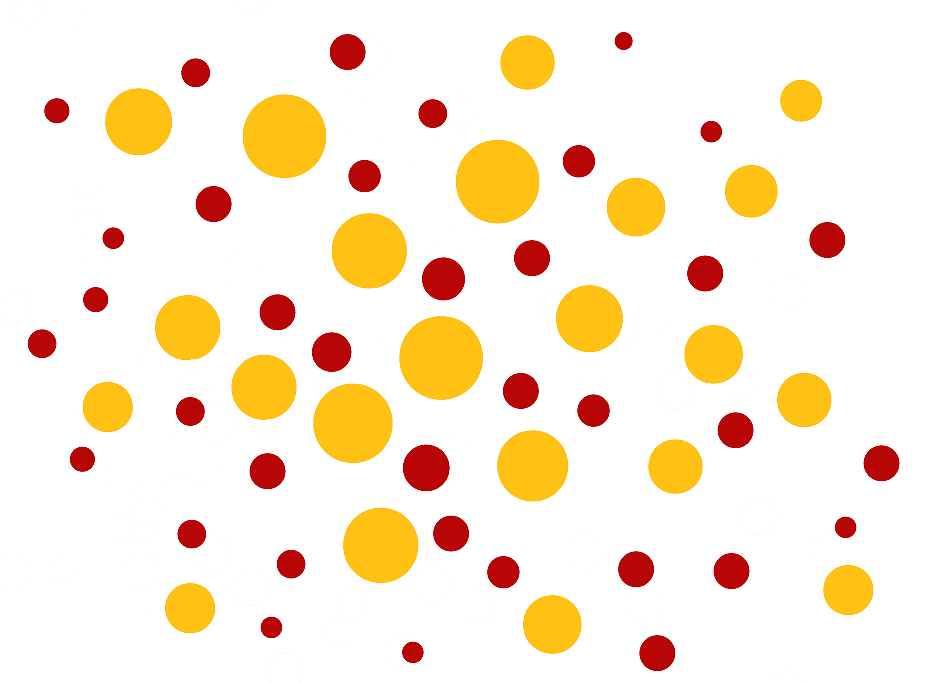
\includegraphics[width=0.3\columnwidth]{figures/Model_FFC.pdf}
SPP:    ~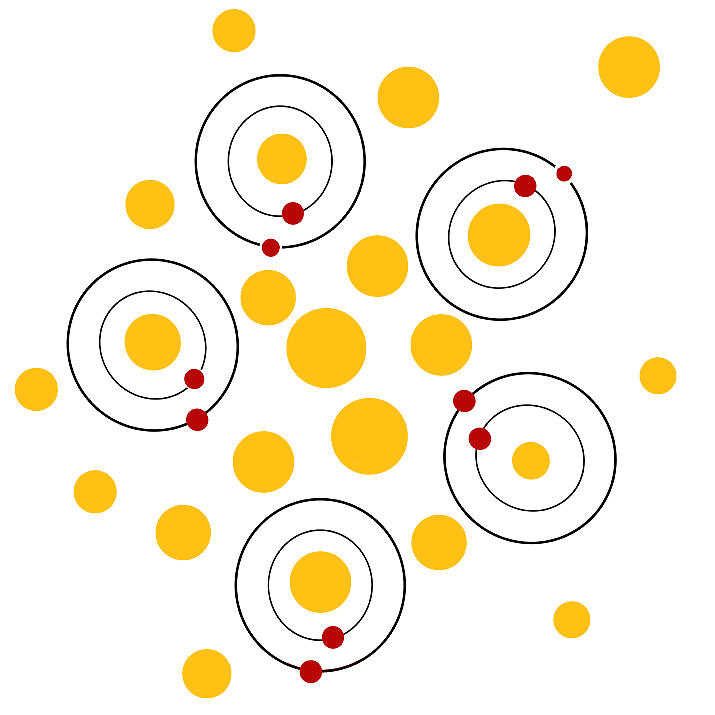
\includegraphics[width=0.25\columnwidth,angle=90]{figures/Model_PP.pdf}\\
SPM:    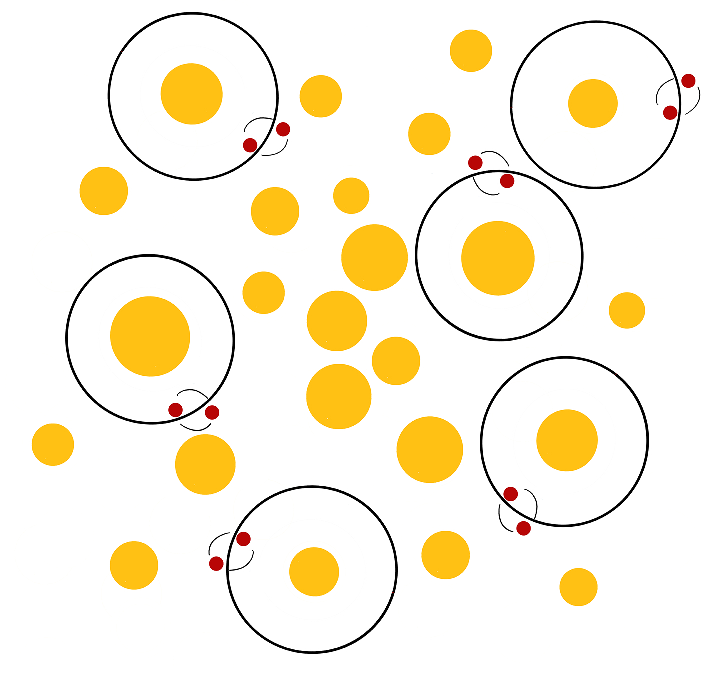
\includegraphics[width=0.25\columnwidth]{figures/Model_PM.pdf}
ISF:    ~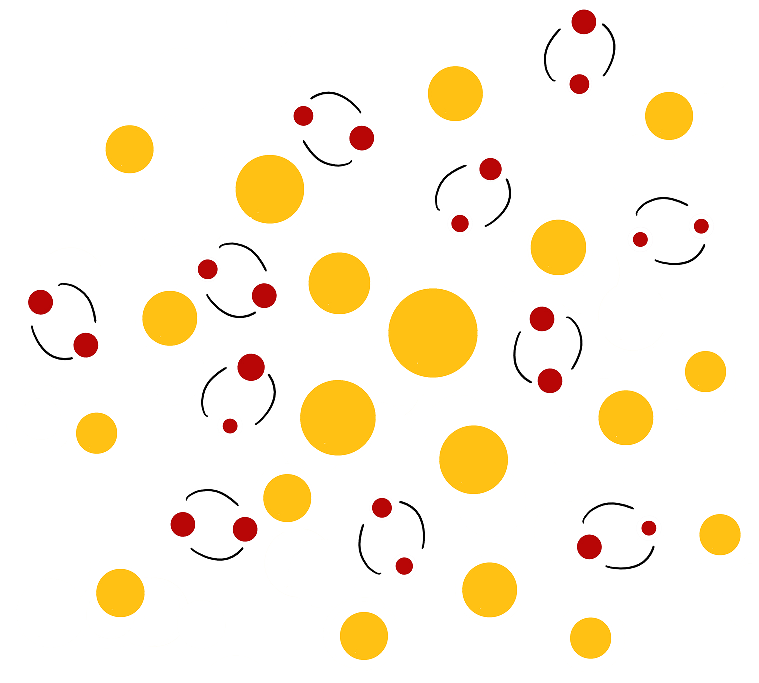
\includegraphics[width=0.3\columnwidth]{figures/Model_SF_FFC.pdf}
\caption{Illustration of the four configurations for Jupiter-mass
  planets in the stellar cluster.  Stars are represented with yellow
  bullets, and planets in red.  From top left to bottom right we have
  (as indicated): model ${\cal FFC}$ for the free floating single
  planets; ${\cal SPP}$ for outer orbiting planets; ${\cal SPM}$ as
  bound planet-moon pair orbiting a star, and model ${\cal ISF}$ in
  situ formation of jumbos.}
\label{Fig:models}
\end{center}
\end{figure}

\subsection{The simulations}\label{Sect:Simulations}

All calculations are performed using 4-th order prediction-correction
direct $N$-body integrator {\sc ph4} \cite{2022A&A...659A..86P}
through the Astrophysical MUltipurpose Software Environment, or AMUSE
for short
\cite{2013CoPhC.183..456P,2013AA...557A..84P,2018araa.book.....P}.
The data files are stored in {\sc AMUSE} formatted particle sets, and
available via zenodo \url{10.5281/zenodo.10149241}; the source
code is available at github \url{https://github.com/spzwart/JuMBOs}.

The script to run the simulations is fairly simple.  It is essentially
the same script from chapter 2 in \cite{2018araa.book.....P},
including the collision-detection stopping condition.  Runs are
performed with the default time-step parameter $\eta=0.03$, which
typically leads to a relative energy error $<10^{-8}$ per step, and
$\aplt 10^{-5}$ at the end of the run. The fractal initial conditions
with small virial radius (0.25\,pc) are, not surprisingly, the hardest
runs to perform. The energy error in these runs can be somewhat higher
at times, but never exceed $<10^{-3}$, which according to
\cite{2041-8205-785-1-L3}, suffices for a statistically reliable
result.  Snapshots were stored every 0.1\,Myr, and the simulations
were continued until 1.1\,Myr, but we analyse the data at an age of
1\,Myr.

Although incorporating stellar evolution, general relativity and the
Galactic tidal field would be straightforward in the AMUSE framework,
we decided to ignore those processes.  We do not expect any stars to
effectively lose much mass during the short duration of the
simulations. Incorporating general relativity would have made the
calculations expensive without much astrophysical gain, and the tidal
field has hardly any influence on the close encounter dynamics in the
cluster central portion.  On the other hand, in the observations,
\jumbos\, seem to be confined towards to the cluster central region.
This, however, is in part an observational selection effects, as it is
difficuly to identify Jupiter-mass objects away from the cluster
center due to intercluster extinction and the lower coverage at the
periphery (S.\, Pearson, private communication).

\subsection{Finding \jumbos}

\jumbos\, are soft in terms of the average local kinetic energy of the
surrounding objects (stars and planets), and this makes them somewhat
hard to find in the numerical models.  One generally consider hard
binary paris or multiples in direct N-body simulations and finding
those soft pairs requires some extra effort.  We search for \jumbos\,
by first selecting any object in the cluster, star or planet, find
the nearest neighbors, and determine their binding energy. If one of
these companions has another object as bound nearests neighbor, we
adopt that as the close pair, and the initially selected object as the
tertiary. Later, we order the particles in terms of distance and
binding energy, on which the eventual designation is based.

Instead of identifying \jumbos\, as bound pairs, we also analyse the
data with just the nearest neighbors using connected components. With
this method we do not establish \jumbos\, as bound objects, but as
close pairs. This second method is to mimic the observations, in which
boundness cannot yet be established.

We recognize single stars $s$, and planets $p$ (although we are
uncertain weather or not to call these objects planets). Pairs of
objects are then placed in parenthesis, for binary stars we write
$(s,s)$, a planetary system with one planet can be $(s,p)$.  A system
with two planets then either becomes $((s,p),p)$, for a hierarcy of
planets, or $(s,(p,p))$ for a planet pair orbiting a star as in the
${\cal SPM}$ model. A \jumbo\, in this nomenclature becomes $(p,p)$.

\section{Results}\label{Sect:Results}

The main results of the calculations are presented in
table\,\ref{Tab:model_numbers} and
table\,\ref{Tab:orbital_distributions}, but also in the more
fine-tuned simulations presented in table\,\ref{Tab:Final_ISF_FFC_Results}.

The large parameter space of how to distribute JMO's among stars, we
start by covering part of this space with a selection of simulations
in which we vary the way JMOs and \jumbos\, are distributed among the
stars. In addition, we cover a small portion of the cluster parameter
space, including the virial radius and the density profile. All the
other parameters we keep constant.

The results of these simulations are reported in
section\,\ref{sect:model_selection}, and in the
tables\,\ref{Tab:model_numbers} and \ref{Tab:orbital_distributions} in
section\,\ref{sect:finetuningbinary_fraction}.

In section\,\ref{sect:ISF_explored} we further explore our favorite
model in which \jumbo\, form as isolated pairs together with the
stars.

\subsection{Distinghuising between the various models}\label{sect:model_selection}


In table\,\ref{Tab:model_numbers} we list per model the number of
different outcomes.  The various simulation results are named after
their model designation followed by either the letter ``Pl'' for the
Plummer model, or ``Fr'' for the Fractal model.  The model name ends
with the virial radius ``R'' in parsec, here R025 indicates 0.25\,pc,
R050 for 0.5\,pc and R100 for 1\,pc virial radius.

\begin{table}
  \caption{The average number of systems per simulations model
    categorized in groups.  The possible outcomes are the number of
    single stars ($n_{s}$), binaries ($n_{(s,s)}$), star orbited by a
    single planet ($n_{(s,p)}$), star orbted by two planets
    ($n_{((s,p),p))}$), single isolated planets ($n_{p}$) and
    \jumbos\, ($n_{(p,p)}$).  Note that we only list those objects
    with a mass $>0.8$\,\MJup.  As a consequence, the total number of
    planary mass objects does not always add up to 600.  The number of
    stars also does not always adds up to 2500 because of collisions
    and hierarchies not listed in the table (see
    section\,\ref{Sect:collisions}).}
 \label{Tab:model_numbers}
 \centering 
 \begin{tabular}{lrrrrrrrrrrrr}
   \hline\hline
   model & $n_{s}$ & $n_{(s,s)}$ & $n_{(s,p)}$ & $n_{((s,p),p))}$ & $n_{p}$ & $n_{(p,p)}$ \\
  \hline
${\cal FFC}$\_Pl\_R025 &  2271 & 87 & 11 & 0 & 580 & 0 \\
${\cal FFC}$\_Pl\_R050 &  2313 & 83 &  3 & 0 & 595 & 0 \\
${\cal FFC}$\_Pl\_R100 &  2331 & 75 &  5 & 0 & 593 & 0 \\
${\cal FFC}$\_Fr\_R025 &  2280 & 93 & 11 & 0 & 584 & 0 \\
${\cal FFC}$\_Fr\_R050 &  2336 & 74 &  4 & 0 & 592 & 0 \\
${\cal FFC}$\_Fr\_R100 &  2312 & 85 &  5 & 0 & 594 & 0 \\
  \hline
  \hline \vspace{-0.75em}\\
${\cal SPP}$\_Pl\_R025 &  2287 &  0 & 84 & 129 & 258 & 0 \\
${\cal SPP}$\_Pl\_R050 &  2224 &  1 & 42 & 232 &  93 & 0 \\
${\cal SPP}$\_Pl\_R100 &  2204 &  0 & 19 & 277 &  26 & 0 \\
${\cal SPP}$\_Fr\_R025 &  2308 & 72 &  8 &   0 & 591 & 0 \\  
${\cal SPP}$\_Fr\_R050 &  2279 & 83 & 28 &   6 & 560 & 0 \\ 
${\cal SPP}$\_Fr\_R100 &  2327 & 64 & 27 &  10 & 553 & 0 \\
  \hline
  \hline \vspace{-0.75em}\\
${\cal SPM}$\_Pl\_R025 &  2480 &  0 & 17 &  3 & 413 & 18 \\
${\cal SPM}$\_Pl\_R050 &  2457 &  0 & 36 &  7 & 341 & 44 \\
${\cal SPM}$\_Pl\_R100 &  2464 &  0 & 22 & 14 & 394 & 15 \\
${\cal SPM}$\_Fr\_R025 &  2320 & 76 &  1 &  0 & 448 &  5 \\ 
${\cal SPM}$\_Fr\_R050 &  2293 & 90 &  2 &  0 & 444 & 17 \\
${\cal SPM}$\_Fr\_R100 &  2361 & 61 &  3 &  0 & 447 & 26 \\
  \hline
  \hline \vspace{-0.75em}\\
${\cal ISF}$\_Pl\_R025 &  2498 & 0 & 0 & 0 & 425 & 23 \\
${\cal ISF}$\_Pl\_R050 &  2498 & 1 & 0 & 0 & 362 & 48 \\
${\cal ISF}$\_Pl\_R100 &  2500 & 0 & 0 & 0 & 246 & 108 \\
${\cal ISF}$\_Fr\_R025 &  2334 & 53 & 7 & 0 & 392 & 0 \\
${\cal ISF}$\_Fr\_R050 &  2309 & 81 & 7 & 0 & 450 & 4 \\
${\cal ISF}$\_Fr\_R100 &  2345 & 73 & 0 & 1 & 454 & 6 \\
  \hline
 \end{tabular}
\end{table}

The ${\cal SPP}$ and ${\cal FFC}$ models systematically fail to
reproduce the observed population of \jumbos\, by a factor of 50 to
400. Changing the initial distribution in semi-major axis of the inner
orbit from a uniform distribution to a logarithmic distribution
reduces the formation rate of \jumbos\, even further.  There are
several systematic trends in terms of cluster density and Plummer
versus fractal distribution, but it is not clear how these models can
lead to \jumbos. Both models produce a considearble population of
binary stars and single planetary systems, in particular in the
fractal distributions, where the typical fraction of dynamically
formed binary stars is around 4\,\%, and the fraction of JMO's
captured by a star is 0.7\,\% per star.  Interestingly, the model that
already start with some paired configuration with a star tends to
produce more binaries and planetary systems, that the models where
planet-mass objects do not orbit stars.  The high abunance of
hierarchical multiple planets, $((s,p),p)$, in the ${\cal SPP}$\_Pl
and ${\cal SPM}$\_Pl models reflects some of the initial
conditions. These models also tend to produce a relatively rich
population of single planet systems $(s,p)$.

The only models that produce a considerably population of \jumbos\,
are the ${\cal SPM}$ models and the ${\cal ISF}$. Where for the latter
the Plummer distributions tend to produce sufficient number of
\jumbos\, whereas the fractal model produce too few.

Rather than directly investigating the orbital separattions, in
figure\,\ref{Fig:twopoint_correlation_ISF_Fr050} we present the
distribution of nearest mutual distance between stars and JMOs for
model ${\cal ISF}$\_Fr\_R050.  Model ${\cal ISF}$\_Pl\_R050 shows
similar trends, but less pronounced.  Note there for calculating the
nearest mutual distance we treated all \jumbos\, as two separate JMO.
This gives rise to the left shoulder in the blue curve in
figure\,\ref{Fig:twopoint_correlation_ISF_Fr050}. This shoulder is
also visible in the star-star curve (black), at a higher elevation
above $\sim 100$\,au, but below a few tens of au JMO-JMO pairs are
relatively more abundant.  The distribution for the mutual distance
between stars and JMOs does not show such a pronoundced shoulder, and
for distances $r_{ij} \apgt 10^4$\,au both distributions converge.

\begin{figure}
    \centering
        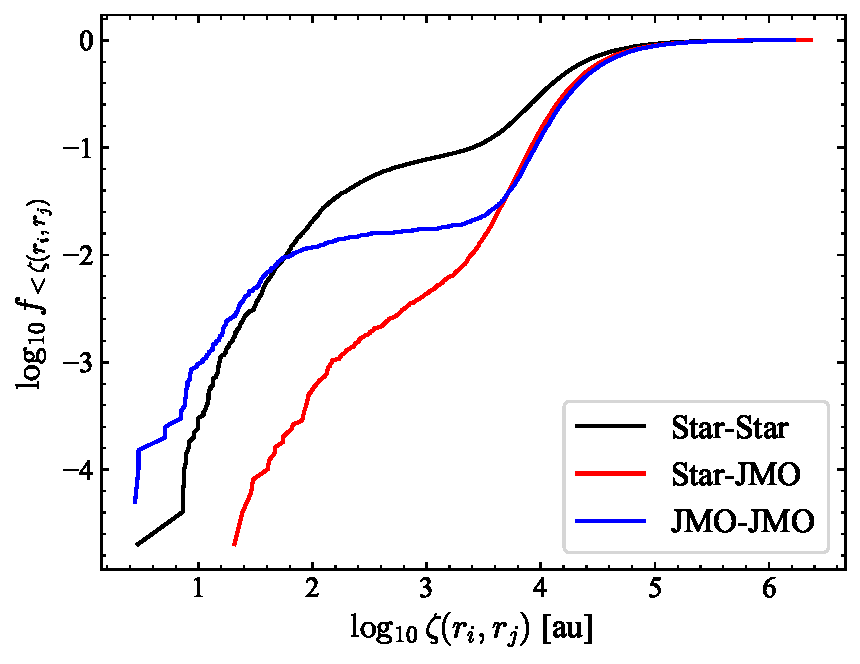
\includegraphics[width=0.75\columnwidth]{figures/two_point_corrFractal_rvir0.5_jmo.pdf}
        \caption{Mutual nearest neighbor distribution function for
          model ${\cal ISF}$\_Fr\_R050. Each object star or JMO is
          treated as separate, and then we establish distributions for
          the mutual nearest neighbor distance for pairs of stars,
          pairs of JMOs and for the distance between a star and a JMO.
          \erwan{ This is the best figure in the paper. Could you make
            a version with added dotted lines for the Plummer model
            R050?}}
        \label{Fig:twopoint_correlation_ISF_Fr050}
\end{figure}

Having established the existence of an overpopulation of nearest
neigbors among stars and JMOs, we further explore the orbital
characteristics of the surviving \jumbos.  The median, the 25\% and
75\% quartiles for the \jumbo, $(p,p)$, distribution for primary mass,
secondary mass, semi-major axis and eccentricity are presented in
table\,\ref{Tab:orbital_distributions}.  The models that produce too
few \jumbos\, to calculate the median and quartiles are omitted.  We
adopt the medial values with the quarlites as realiable interval for
comparing the observational data with the simulations because the
distributions are rather skewed. This is noticeable in the large
difference between the sizes of the lower and the upper quartiles.


\begin{table*}
  \caption{Simulation results for the models that produce a
    sufficiently large population of \jumbos\, to be considered
    feasable (mainly models ${\cal SPM}$ and ${\cal ISF}$). We present
    the median values and the quartile intervales for 25\,\% and
    75\,\%.  The observed median inter-JMO distance in the Trapezium
    cluster is $r_{ij} = 193.8^{+78.2}_{-114.1}$\,au $M_{\rm prim} =
    3.67^{+1.31}_{-1.57}$\,\MJup, and $M_{\rm sec} =
    2.10^{+1.05}_{-1.05}$\,\MJup\, \cite{2023arXiv231001231P}.  }
\label{Tab:orbital_distributions}
 \centering 
 \begin{tabular}{llllll}
 \hline\hline
model&$\langle M \rangle$/\MJup & $\langle m \rangle$/\MJup & $\langle a \rangle$/au & $\langle e \rangle$ \\
 \hline \vspace{-0.75em} \\ 
 ${\cal SPM}$\_Pl\_R025 & $3.62^{+1.36}_{-2.68}$ & $1.12^{+0.24}_{-2.14}$ & $99.08^{+37.24}_{-36.38}$ & $0.47^{+0.18}_{-0.13}$ \\
 ${\cal SPM}$\_Pl\_R050 & $4.02^{+2.10}_{-3.71}$ & $1.74^{+0.73}_{-0.93}$ & $94.28^{+32.78}_{-78.90}$ & $0.33^{+0.19}_{-0.27}$ \\  
 ${\cal SPM}$\_Pl\_R100 & $6.93^{+4.38}_{-3.07}$ & $1.29^{+0.23}_{-1.22}$ & $140.96^{+37.10}_{-11.20}$ & $0.12^{+0.05}_{-0.27}$ \\
 ${\cal SPM}$\_Fr\_R025 & $2.66^{+1.78}_{-3.20}$ & $1.87^{+1.05}_{-0.37}$ & $35.56^{+20.57}_{-62.84}$ & $0.80^{+0.10}_{-0.18}$ \\ 
 ${\cal SPM}$\_Fr\_R050 & $9.64^{+7.02}_{-1.99}$ & $2.00^{+0.69}_{-0.58}$ & $82.76^{+21.74}_{-83.04}$ & $0.56^{+0.29}_{-0.18}$ \\ 
 ${\cal SPM}$\_Fr\_R100 & $4.60^{+2.57}_{-2.44}$ & $1.80^{+0.64}_{-2.47}$ & $73.20^{+27.21}_{-100.43}$ & $0.38^{+0.21}_{-0.13}$ \\
 \hline \vspace{-0.75em} \\ 
 ${\cal ISF}$\_Pr\_R025 & $8.12^{+3.44}_{-4.51}$ & $2.10^{+0.98}_{-1.66}$ & $112.06^{+40.76}_{-181.76}$ & $0.43^{+0.08}_{-0.19}$ \\
 ${\cal ISF}$\_Pl\_R050 & $7.00^{+3.28}_{-4.23}$ & $2.03^{+0.68}_{-0.99}$ & $296.40^{+168.53}_{-190.04}$ & $0.62^{+0.19}_{-0.12}$ \\
 ${\cal ISF}$\_Pl\_R100 & $5.25^{+2.37}_{-3.16}$ & $1.60^{+0.72}_{-1.40}$ & $457.63^{+265.29}_{-193.56}$ & $0.67^{+0.23}_{-0.14}$ \\
 ${\cal ISF}$\_Fr\_R050 & $4.82^{+3.05}_{-4.42}$ & $1.38^{+0.75}_{-2.42}$ & $37.57^{+15.07}_{-42.46}$ & $0.77^{+0.06}_{-0.05}$ \\  
 ${\cal ISF}$\_Fr\_R100 &$10.15^{+3.75}_{-2.84}$ & $1.98^{+0.50}_{-2.13}$ & $97.05^{+47.34}_{-189.07}$ & $0.77^{+0.17}_{-0.16}$ \\
 \hline \vspace{-0.75em} \\ 
 \end{tabular}
\end{table*}

The primary masses produced in the models ${\cal SPM}$ and ${\cal
  ISF}$, tend to be on the high side, but the secondary masses are in
the observed range.  All the ${\cal SPM}$ models tend to lead to
orbits that are too tight, but omitting the orbits with $a<25$\,au
\jumbos\, does not improve the median orbital separation.  In terms of
the orbital separation (or projected distance) the best model seems to
be ${\cal ISF}$ Plummer with a 0.5\,pc virial radius, but the
distributions are wide, and although the 1\,pc ${\cal ISF}$ fractal
model exhibits a low formation rate, it does reproduce the observed
separation distribution. Note that models ${\cal ISF}$\_Fr at an age
of 0.2 or 0.3\,Myr compare quite fovarably to the observations (see
section\,\ref{Sect:Discussion}).

The eccentricities in model ${\cal SPM}$\_Pl are generally smaller
than in the fractal models.  The planet-moon pairs in those models
started in almost circular orbits.  In the fractal models, the
eccentricities are more effectively perturbed and thermalized, whereas
in the Plummer models this does not happen.  In model ${\cal ISF}$,
\jumbos\, start with higher average eccentricities, in which case de
difference in eccentricity between the Plummer and fractal models is
less pronounced. Later, in section\,\ref{sect:ISF_explored}, we will
explore ${\cal ISF}$ models with initially curcular orbits.

\subsection{Stellar and planetary collisions}\label{Sect:collisions}

We encountered quite a number of collisions in the simulation, but the
majority occur between two stars (83\%), with the rest between a star
and a Jupiter-mass object.  Collisions between two Jupiter-mass
objects are very rare.  Most collisions happen in the fractal models.
In figure\,\ref{Fig:collision_evolution_ISF_Fr} we present the
cumulative distribution of collisions in the models {\cal ISF}\_Fr
with a virial radius of 0.25\,pc (solid blue), 0.5\,pc (orange) and
1.0\,pc (green), and for the equivalent models {\cal FFC}\_Pl with the
thin dash-dotted curves.  The higher density naturally leads to more
collisions, and those collisions tend to occur earlier in time.  

Plummer models tend to lead to fewer collisions.  The only Plummer
models in which collisions among stars were common is in model ${\cal
  FFC}$ with 64, 20 and 18 collisions on average per cluster, for
those models with a viral radius of 0.25\,pc, 0.5\,pc and 1.0\,pc,
respectively.  Interestingly enough, the fractal models from the same
series only experience 30, 17 and 14 collisions for the same virial
radii.  It came as a bit of a surprise that models ${\cal FFC}$\_Pl
lead to so many collisions, even though no collisions happen between
two Jupiter-mass objects.

\begin{figure}
\centering
    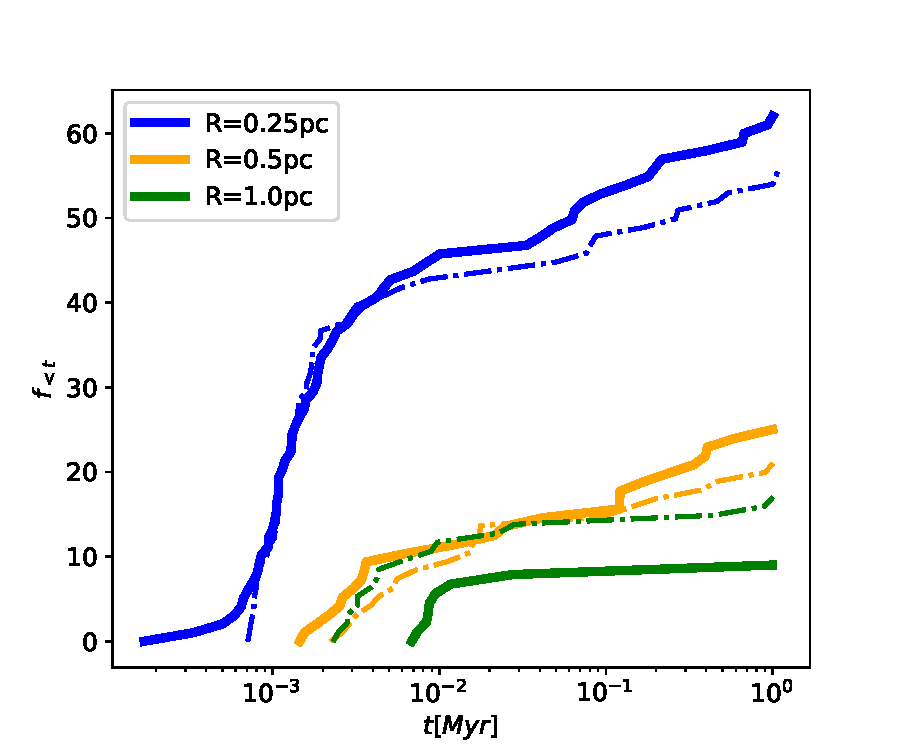
\includegraphics[width=0.75\columnwidth]{figures/fig_collision_evolution_ISF_Fr.pdf
    }
        \caption{Number of collisions as a function of time for model
          ${\cal SPM}\_Fr$ (solid lines) and for models ${\cal
            FFC}\_Pl$ (dash-dotted lines).}
         \label{Fig:collision_evolution_ISF_Fr}
\end{figure}

\subsection{Runaway \jumbos}

In addition to mergers, ejection events also occurred.  We adopt the
classical definition of identifying runaway objects if their velocity
with respect to the center of mass of the entire stellar system
(dominated by the bound cluster) exceeds 30\,km/s
\cite{1961BAN....15..265B}.

Not surprisingly, no \jumbo\, escaped the cluster with a high
velocity, but there are some slow runaways, which were born in the
cluster periphery and never experienced an encounter with a nearby
star. Adding a tidal field to our calculations may cause this
population to increase.

Single runaway stars and JMOs are also rare in our simulations. We
attribute this rareness to the lack of hard binaries in the initial
conditions.  We encounter on average one runaway JMO for each of the
fractal models, and typically twice as many runaway stars.  The JMOs,
however have on average a velocity of $110$\,km/s, whereas the stars
escape with $\sim 63.3$\,km/s.

\subsection{Fine-tuning for the binary fraction and separation distribution}\label{sect:finetuningbinary_fraction}

Having established that we prefer model ${\cal ISF}$, we will further
explore the consdequences, and try to derive some of the earlier
\jumbo\, properties to see if those are reconcilable with our
understanding of planet and star-formation in
section\,\ref{sect:ISF_explored}.

In figure\,\ref{Fig:Fjumbo_vs_time_model_ISF_Fr} we illustrate how the
fraction of jumbos\, rapidly decreases with time in models ${\cal
  ISF}$\_Pl\_R050 and ${\cal ISF}$\_Pl\_R100 (and the equivalent
fractal models) for the light blue and red curves.  The binary
fraction among jupite-mass objects initially drops quickly (even
exponentially in the fractal models), to slow down after $\sim
0.2$\,Myr at a survival fraction of $\sim 2$\,\% for the 0.5\,pc
virial radius and $\sim 10$\,\% for the 1\,pc virial radius
cluster. For the latter model, the fraction of \jumbos\, drops
eventually to about 4\,\%; lower than the observed 8\,\%.

\begin{figure}
    \centering
    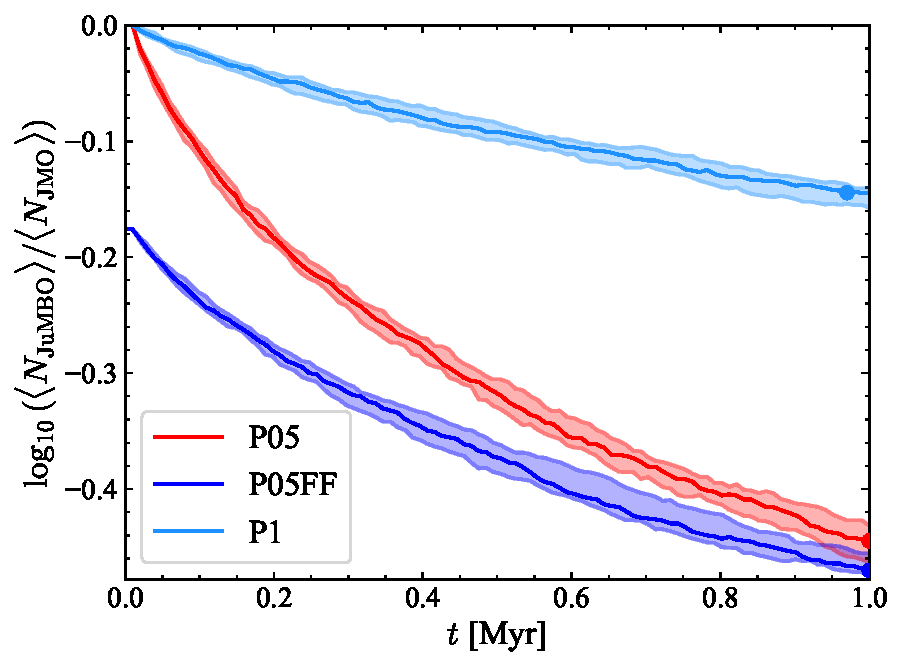
\includegraphics[width=0.49\columnwidth]{figures/Plummer_General_fJuMBO_evol.pdf}
    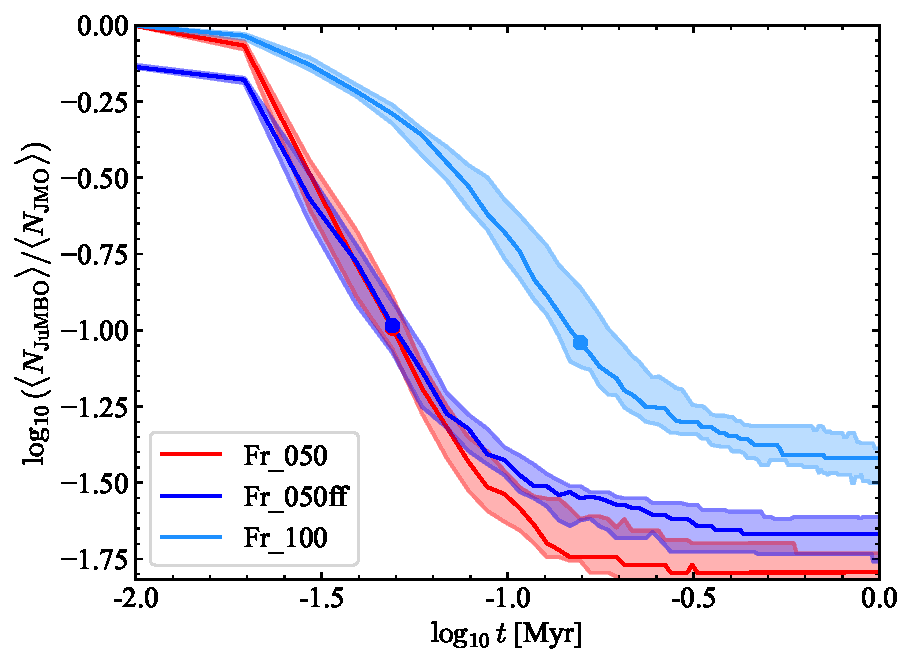
\includegraphics[width=0.49\columnwidth]{figures/Fractal_General_fJuMBO_evol.pdf}
    \caption{Fraction of jumbos as a function of time for models
      ${\cal ISF}$\_Pl\_R050 and ${\cal ISF}$\_Pl\_R100 (left panel,
      with a Plummer initial density profile), ${\cal ISF}$\_Fr\_R050
      and ${\cal ISF}$\_Fr\_R100 (right panel) For model ${\cal
        ISF}$\_Pl\_R050 we also perform a calculation with a
      population of single Jupiter-mass objects. The number of free
      floating objects is the same as the number if primordial
      \jumbos\, and their masses are taken from the primary mass
      function.
}
        \label{Fig:Fjumbo_vs_time_model_ISF_Pl}
        \label{Fig:Fjumbo_vs_time_model_ISF_Fr}
\end{figure}


To investigate the evolution of the mean orbital separation of the
surviving \jumbos, and the effect of changing the initial distribution
in orbital separation, we present
figure\,\ref{Fig:sma_vs_time_model_ISF_Fr}. Here we show how the
distribution in orbital separation of the jumbos\, in model ${\cal
  ISF}$\_Pl\_R050 rapidly drops with time, and converges in $\aplt
0.1$\,Myr to a median separation $<100$\,au. This distribution is much
narroware and on average with a smaller mean than observed in the
Trapezium cluster.

\begin{figure}
  \centering
        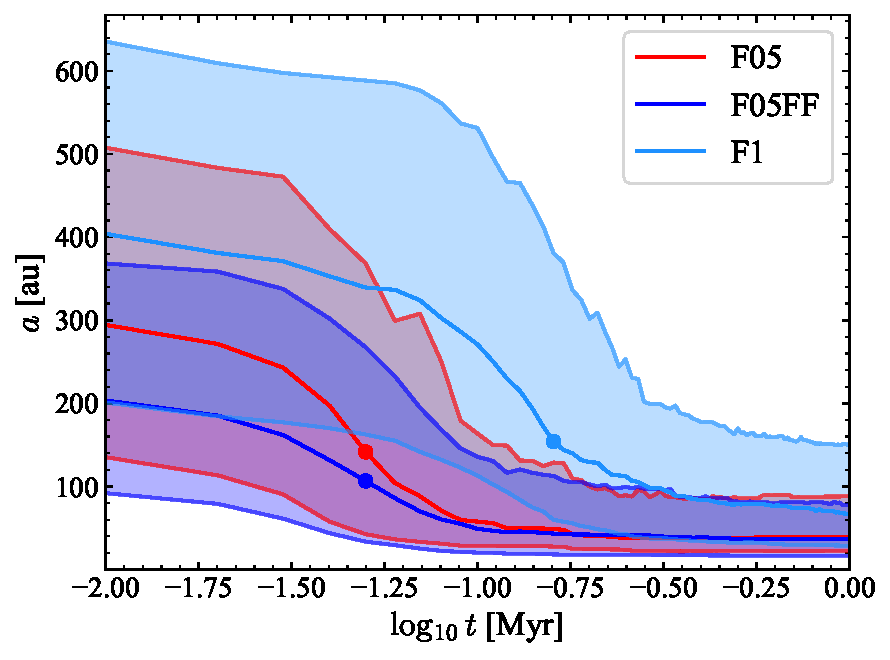
\includegraphics[width=0.75\columnwidth]{figures/Fractal_General_sem_evol.pdf}
        \caption{Evolution of the median orbital separation and the
          20\% and 75\% quartiles of the distribution for model ${\cal
            ISF}$\_Pl\_R050 (red).  In addition we show the model in
          which all \jumbos\, were initially in circular orbits (light
          blue), and the model in which we constain the initial
          separation to 400\,au\, rather than the generally adopted
          1000\,au. }
        \label{Fig:sma_vs_time_model_ISF_Fr}
\end{figure}

We further explore the effect of changing the initial eccentricity or
semi-major axis distribution, but these choices do not seem to make a
sufficienly big difference to salvage the fractal models for
explaining the observed population of \jumbos.  Starting with a
tighter population of \jumbos\, will help delaying their ionization,
but hardly affects the eventual distribution in orbital separation.
On the other hand, it will help in making the fraction of \jumbos\,
consitent with the observations. Such consistency is reached $\sim
0.2$\,Myr or $0.3$\,Myr after the start of the simulations.  At this
time, the fraction of \jumbos\, to JMOs as well as the separation
distribution of the surviving \jumbos\, are consistent with the
observed population. We consider this a strong argument in favor of
\jumbos\, as late formed objects.

In figure\,\ref{Fig:sma_vs_time_model_ISF_FrA} we present the orbital
distribution for \jumbos\, in model ${\cal ISF}$\_Fr050 (with and
without free floating JMOs) at a age of 0.2\,Myr. Shortly after the
\jumbos\, are introduced in the simulation, the widest orbits are
being ionized, and by the time the cluster reaches an age of 1.0\,Myr,
the orbital distribution is skewed too much to lower values, compared
to the observations. AT this age, however, the numbre of \jumbos\, as
well as their orbital separations matches the observed populations in
the Trapezium cluster. 

\begin{figure}
    \centering
    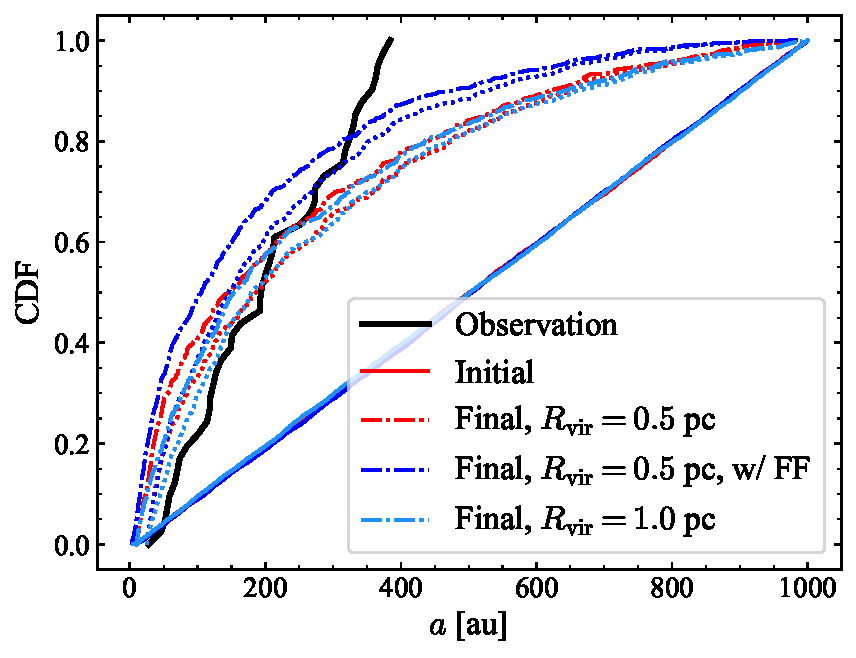
\includegraphics[width=\columnwidth]{figures/Fractal_General_sem_axis_crop.pdf}
    \caption{
      \erwan{Let's get rid of the dotted curves; reduces also the legend. Still need a caption. change CDF.}  }
        \label{Fig:sma_vs_time_model_ISF_FrA}
\end{figure}


\subsection{Introducing a population of free floaters in model ${\cal ISF}$}\label{sect:ISF_explored}

With the current models, we can further constrain the simulation
parameters by repeating several calculations for better statistics and
exploring other parts of the parameter space.  We perform this
analysis for model ${\cal ISF}$, because that model seems most
promising for producing a sufficiently large population of \jumbos\,
in the range of observed parameters.

The orbital distribution of the surviving \jumbos\, in the Plummer
models is considerably more satisfactory than those that survive the
fractal models (see figure\,\ref{Fig:Gen_Semi_Fractal}). The tail to
wider orbits, however, is more pronounced, potentially highlighting
problems with initial conditions.
Reducing the maximum orbital separation from 1000\,au to 400\,au helps
resolving this discrepancy, but it seems a bit unfair to tune the
initial conditions to mimick the observed parameters if the majority
of primordial \jumbos\ survives. It would be relatively
straightforward to acquire a satifcatory comparison between
simulations and observations if we start the simulations with a
population of \jumbos\, that reflects the observations.

Using the results of the models from
section\,\ref{sect:model_selection}, we alter our initial conditions
with the aim of mimicking observations. Doing so allows us to
disentangle aspects of the cluster history, allowing for predictions
on the properties of \jumbo\, formation.

We performed several simulatons with a virial radius of 0.5\,pc and
1.0\,pc and for Plummer as well as for fractal models. Some models
were run with an additional population of single JMO's. In those
cases, we often chose to have an equal number of JMO's as \jumbos.
The masses of these free floaters is identical to the \jumbo\,
primaries, and they are distributed in the same density profile.
These models, different from the ${\cal FFC}$ in that they still have
a population of \jumbos\, at the start. Each model calculation was
repeated 10 times in order to build up a more reliable statistical
sample.

For all models, we constrain $n_{\mathrm{\jumbo}} + n_{\mathrm{FF}}$
to values reflecting the total planetary-mass population observed in
\cite{2023arXiv231001231P}, keeping in mind the survival rate of
\jumbos\, based on previous results to decide on the initial value of
$N_{\mathrm{\jumbo}}$. The range of primary and secondary masses is
adapted to a flat distribution in masses in contrast to the power-law
mass function in our earlier models (see
section\,\ref{Sect:Model}). The semi-major axis is uniformly
distributed between the restricted range $a\in[25,100]$ au, which is
somewhat narrower than we adopted before in section\,\ref{Sect:Model}.
We run an additional series of simulations in which the primordial
\jumbos\, have an eccentricity beween 0.0 and 0.2 sampled from a
uniform distribution, rather than the usual thermal eccentricity
distribution.  For the models that include free floating JMO's we add
the designation ``ff'' to the model name, and the circular models
recieve a letter 'c', for circular.  The results of this series of
${\cal ISF}$ model calculations are summarized in table
\ref{Tab:Final_ISF_FFC_Results}.
      
\begin{table*}
         \caption{Statistics on the surviving \jumbos. $\langle
           ...\rangle$ gives the median, while the $\pm$ denote where
           the lower and upper quartiles. Col. 1: The fraction of
           \jumbos\, present at the end of the simulation relative to
           the number initialised. Col. 2: The fraction of \jumbos\,
           with projected separation, $r_{\mathrm{ij}} > 25$
           au. Col. 3: The mass ratio of \jumbo\, systems. Col. 4: The
           primary mass of the \jumbo\, system. Col. 5: The semi-major
           axis of the \jumbo\, system. Col. 6: The eccentricity of
           the system.
           \erwan{should we get of the second column. Also, the caption needs work. I can do that.}
           }
        \label{Tab:SF_Res}
        \centering 
        \begin{tabular}{c c c c c c c c c}
        \hline\hline
        Model & $f_{\mathrm{surv}}$ & $f_{r_{ij} \geq 25\mathrm{ au}}$ & $\langle M_{\mathrm{prim}} \rangle\ [M_{\mathrm{Jup}}]$ & $\langle M_{\mathrm{sec}} \rangle\ [M_{\mathrm{Jup}}]$ & $r_{ij}$ [au] &$\langle a \rangle$ [au] & $\langle e \rangle$\\
        \hline \vspace{-0.75em}\\ 
           Pl\_050     & $0.37^{+0.01}_{-0.02}$ & $0.94^{+0.02}_{-0.01}$ & $8.3^{+2.7}_{-3.1}$ & $3.6^{+2.7}_{-1.8}$ & $233^{+234}_{-137}$ & $268^{+237}_{-152}$ & $0.68^{+0.16}_{-0.22}$ \vspace{0.25em}\\
           Pl\_050ff   & $0.52^{+0.02}_{-0.00}$ & $0.92^{+0.00}_{-0.01}$ & $8.1^{+2.8}_{-3.2}$ & $3.4^{+2.7}_{-1.7}$ & $162^{+167}_{-94}$ & $187^{+176}_{-106}$ & $0.61^{+0.14}_{-0.18}$ \vspace{0.25em}\\
           Pl\_100      & $0.72^{+0.02}_{-0.01}$ & $0.97^{+0.00}_{-0.01}$ & $7.8^{+3.0}_{-3.0}$ & $3.3^{+2.5}_{-1.6}$ & $344^{+271}_{-188}$ & $396^{+250}_{-206}$ & $0.68^{+0.16}_{-0.20}$ \vspace{0.25em}\\
           Fr\_050     & $0.02^{+0.00}_{-0.00}$ & $0.67^{+0.19}_{-0.07}$ & $8.6^{+2.4}_{-3.3}$ & $4.2^{+3.2}_{-1.9}$ & $38^{+52}_{-18}$ & $39^{+50}_{-16}$ & $0.67^{+0.16}_{-0.19}$ \vspace{0.25em}\\
           Fr\_050ff   & $0.04^{+0.00}_{-0.01}$ & $0.61^{+0.02}_{-0.11}$ & $8.8^{+2.7}_{-2.6}$ & $3.9^{+2.5}_{-2.0}$ & $30^{+43}_{-16}$ & $37^{+41}_{-20}$ & $0.62^{+0.14}_{-0.21}$ \vspace{0.25em}\\
           Fr\_100      & $0.04^{+0.00}_{-0.01}$ & $0.72^{+0.11}_{-0.06}$ & $8.3^{+2.4}_{-3.0}$ & $3.8^{+2.4}_{-1.9}$ & $64^{+98}_{-40}$ & $67^{+83}_{-38}$ & $0.68^{+0.16}_{-0.19}$ \vspace{0.25em}\\
           Fr\_050ffL  & $0.03^{+0.00}_{-0.00}$ & $0.46^{+0.07}_{-0.07}$ & $8.1^{+2.9}_{-2.7}$ & $2.7^{+3.1}_{-1.0}$ & $33^{+20}_{-18}$ & $20^{+15}_{-9}$ & $0.61^{+0.20}_{-0.19}$ \vspace{0.25em}\\
           \hline \vspace{-0.75em}\\
           Pl\_050ffO  & $0.76^{+0.01}_{-0.01}$ & $0.89^{+0.03}_{-0.03}$ & $3.7^{+3.5}_{-2.1}$ & $2.1^{+2.5}_{-1.2}$ & $90^{+86}_{-44}$ & $105^{+86}_{-47}$ & $0.61^{+0.15}_{-0.17}$ \vspace{0.25em}\\
           Pl\_050O    & $0.02^{+0.00}_{-0.01}$ & $1.00^{+0.00}_{-0.16}$ & $4.0^{+2.6}_{-1.9}$ & $2.8^{+1.7}_{-1.5}$ & $61^{+46}_{-24}$ & $67^{+48}_{-22}$ & $0.67^{+0.14}_{-0.19}$ \vspace{0.25em}\\
           Fr\_050ffO  & $0.03^{+0.00}_{-0.00}$ & $0.8^{+0.02}_{-0.15}$ & $3.4^{+3.4}_{-1.7}$ & $1.8^{+2.0}_{-0.8}$ & $44^{+37}_{-18}$ & $46^{+38}_{-22}$ & $0.69^{+0.15}_{-0.18}$ \vspace{0.25em}\\
           Fl\_050OC   & $0.02^{+0.01}_{-0.00}$ & $0.67^{+0.19}_{-0.07}$ & $4.7^{+3.2}_{-2.7}$ & $3.6^{+2.6}_{-2.02}$ & $46^{+36}_{-26}$ & $49^{+28}_{-28}$ & $0.45^{+0.33}_{-0.23}$ \vspace{0.25em}\\
           \hline
         \hline                                   %inserts single line
         \label{Tab:Final_ISF_FFC_Results}
        \end{tabular}
     \end{table*}

Adding a population of free floaters to the Plummer models, makes
considerable difference in the evolution of the \jumbo\, fraction, but
eventually, after about 1\,Myr their fraction converges to roughly the
same value.  For models ${\cal ISF}$\_Pl\_R050 and ${\cal
  ISF}$\_Fr\_R050, illustrated in
figure\,\ref{Fig:Fjumbo_vs_time_model_ISF_Fr}, this additional
population of free floaters makes a considerable difference in the
binary survival rate (see table\,\ref{Tab:SF_Res}).

It does make a difference in the orbital distribution of \jumbos\,
though, becasue the interaction between a relatively tight\jumbo\,
with a relatively low-mass JMO could be hard, tightening the \jumbo's
orbit, whereas an encounter with a more massive object either widens
the orbit or dissociates it.

More \jumbos\, survive in the simulations that included a population
of free floating JMOs.  This increased surviveability may be the
result of the hardening of the \jumbos\, by occasional hard encounters
with a JMO, making the former less vulnerable for ionization.  The
consequence of this hardening process is also visible in
figure\,\ref{Fig:Gen_Semi_Plummer} where the \jumbos\, in the models
that included free floaters are on average tighter.  This tightening
of the orbits establishes itself already at a very early age, as can
be seen in figure\,\ref{Fig:sma_vs_time_model_ISF_FrA}.  The \jumbos\,
in these runs, however, remain soft for encounters with any of the
stellar-mass objects in the cluster. The hardening then reduces the
interaction cross section of the \jumbo\, making it less vulnerable
for any interaction, including ionization.

The Fractal distribution efficiently prunes off any wide orbits since
its violent nature provokes many encounters resulting in
ionization. The tendency for \jumbos\, to ionise at any encounter is
reflected by the little variation between runs of the same virial
radius. Also note the tendency for \jumbos\, to ionise even when
encountering a JMO. This is reflected in the models with free floating
JMOs to have smaller orbital separations on average.  This trend is
even more clear in the Plummer models, see
figure\,\ref{Fig:Gen_Semi_Plummer}.  where the orbital separations for
models Pl\_050 $\langle a\rangle\sim296$\,au compared to $\langle
a\rangle\sim187$ au for model Pl\_050ff.

Including free floating JMOs
then lead to more \jumbos\, they have tighter orbits, and the widest
orbits are ionized more effectively.

Increasing the number of JMOs also enhances the chances of two
free-floaters settling into a newly formed binary, on average, only
$0.40$ new \jumbo\, systems emerge in models Fr\_050 compared to the
$0.65$ in Fr\_050ff. For the Plummer models the increased \jumbo\,
formation rate is even more striking by increasing from $1.75$ for
model Pl\_050 to $3.15$ for model Pl\_050ff.  This result shaprly
contrasts the ${\cal FFC}$ models, where, irrespective of how many
JMOs we added to the cluster (up to $10^4$) no \jumbos\, formed in any
of our simulations (see section\,\ref{sect:FFC_model_results} for a
discussions). The primordial presence of \jumbos\, mediates their
further formation through interactions with JMOs.



\begin{figure}
    \centering
    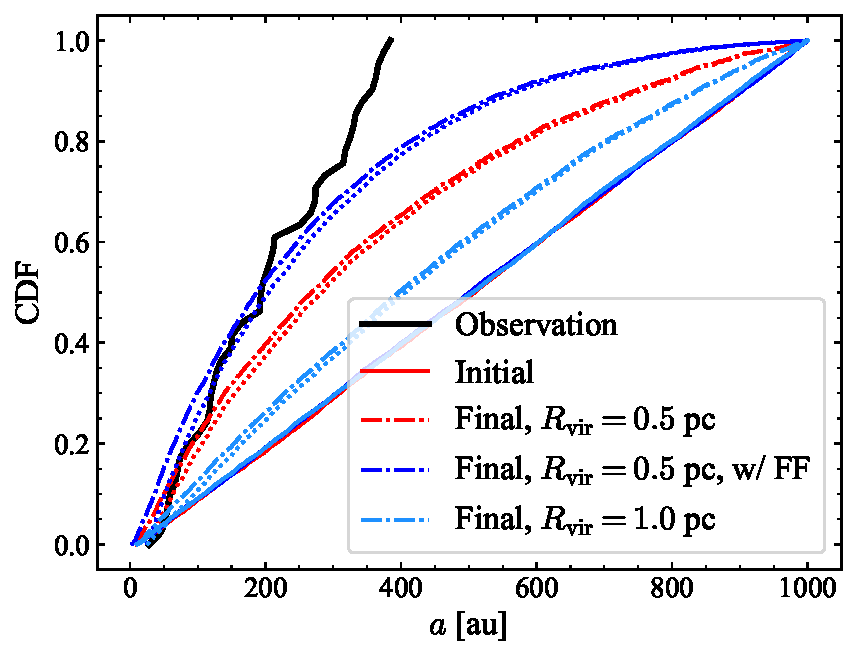
\includegraphics[width=0.49\columnwidth]{figures/Plummer_General_sem_axis.pdf}
    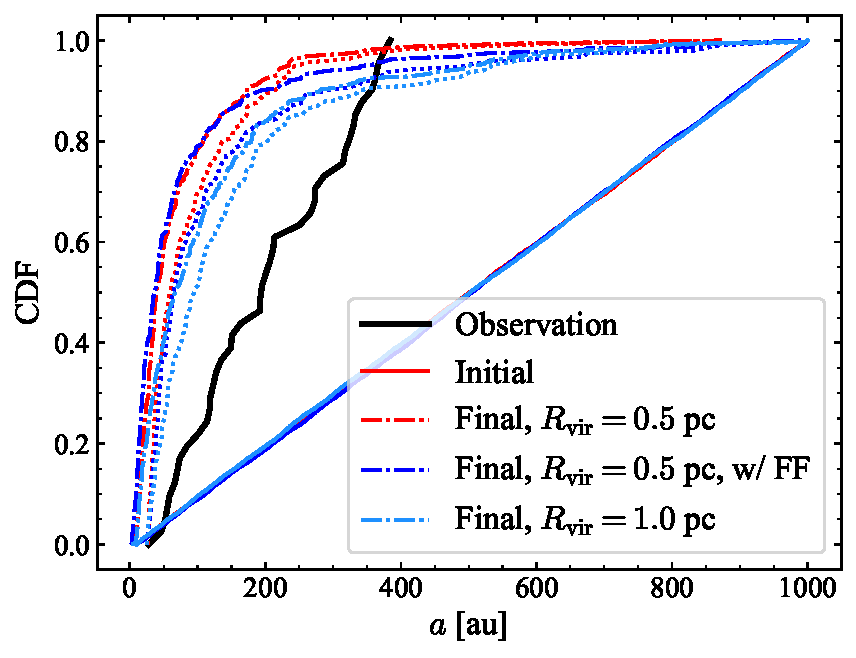
\includegraphics[width=0.49\columnwidth]{figures/Fractal_General_sem_axis.pdf}
    \caption{Cumulative distribution of surviving \jumbo\, semi-major
      axis distribution for models Pl\_050, Pl\_050ff, and Pl\_100
      (left panel), and Fr\_050, Fr\_050ff, Fr\_100 (right panel).
    \erwan{replace the CDF axis labels.}}
    \label{Fig:Gen_Semi_Plummer}
    \label{Fig:Gen_Semi_Fractal}
\end{figure}


\begin{figure}
    \centering
    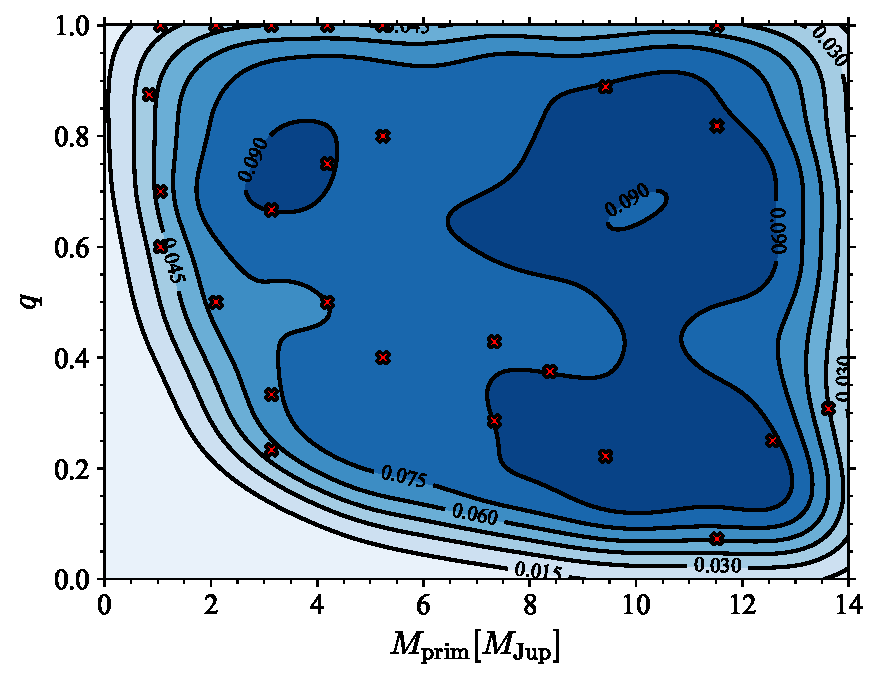
\includegraphics[width=0.49\columnwidth]{figures/Plummer_rvir0.5_FF_mass_distr.pdf}
    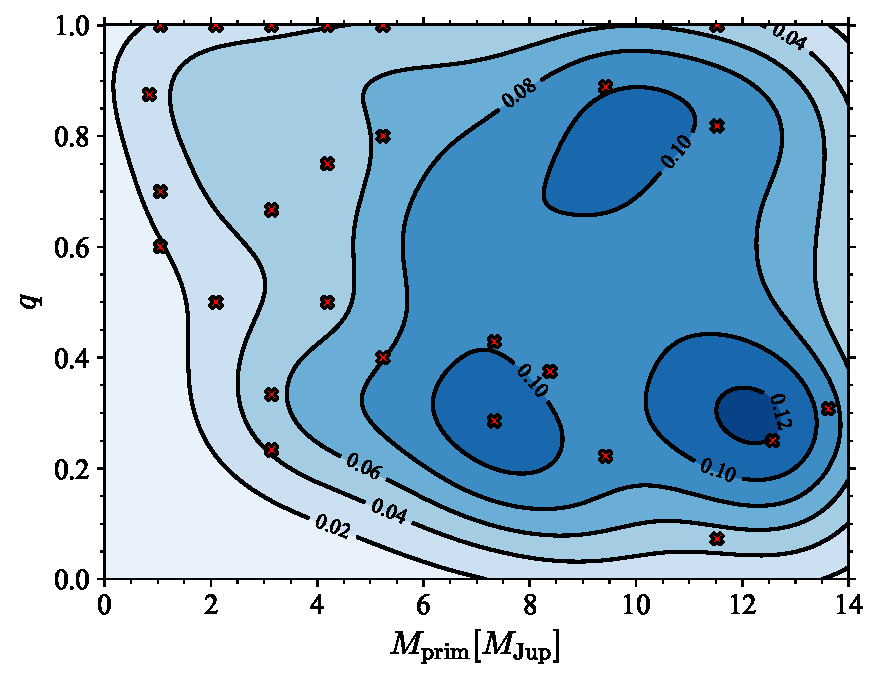
\includegraphics[width=0.49\columnwidth]{figures/Fractal_rvir0.5_FF_mass_distr.pdf}
    \caption{Probability distribution of primary mass versus mass
      ratio for the simulated \jumbos\, in model ${\cal
        ISF}$\_Pl\_R050ff (blue contours).  The red crosses show the
      observed \jumbos.  The primary masses for these runs ware
      generated from a uniform distribution, which is still evident in
      the Plummer model (left), but in the fractal model the initial
      conditions are lost.  }
         \label{Fig:Gen_mdistr_Plummer}
         \label{Fig:Gen_mdistr_Fractal}
\end{figure}

In figure\,\ref{Fig:Gen_mdistr_Plummer} we present the probability
distrution of primary \jumbo\, mass and mass ratio for Plummer and
fractal models.  The observed point (red) seem to cover a similar
parameter space, but overall distribution does not seem to be
consistent with the observations. For the Plummer models this is, in
principle, relatively simple to resolve, but using the observed
distribution as input. For the fractal models such fine-tuning will be
considerably harder because the fraction of survivers is only $\sim
4$\,\%.

The overabundance of equal-mass \jumbos\, at $\aplt 4$\,\MJup\,
primary masses in the observations is quite striking, and hard to
explain. If not just statistics or observational bias, this could
indicate some curious formation mechanism. The high-mass-ratio
population \jumbos\, is further illustrated in
figure\,\ref{Fig:obs_q_mprim_sep}, where we plot the observed \jumbo\,
population (data from \,\cite{2023arXiv231001231P}).

\begin{figure}
    \centering
    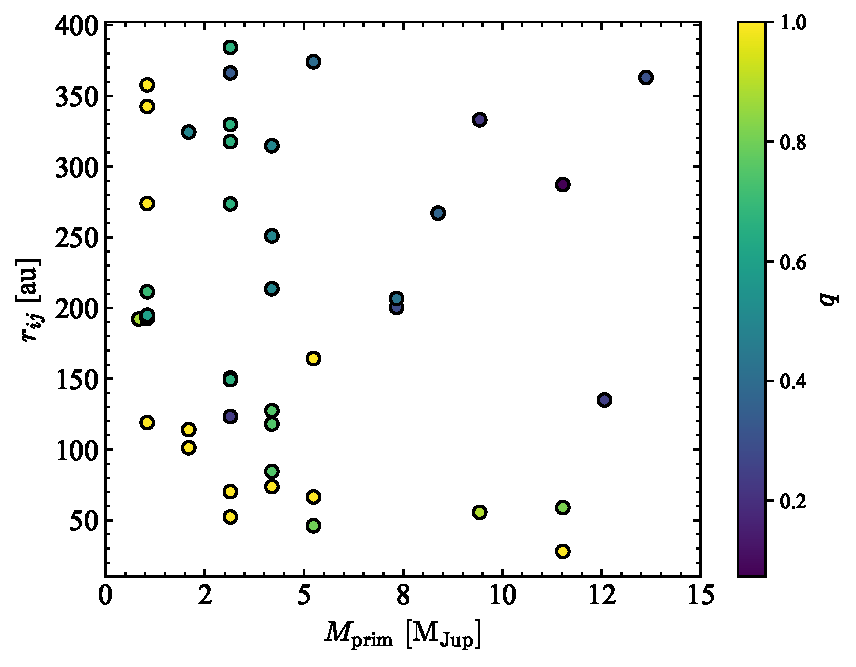
\includegraphics[width=0.75\columnwidth]{figures/obs_q_mprim_sep.pdf}
    \caption{Distribution function of the observed \jumbos, for
      primary mass, observed projected separation and mass-ratio
      (colors). The yellow bullet points indicate the high mass-ratio
      population, whereas the green/blue bullets show the low-mass
      ratio population.
      \erwan{Can you make the symbols larger?}
    }
    \label{Fig:obs_q_mprim_sep}
\end{figure}

We could continue calibrating the initial conditions for a more
consistent comparison with the observations, but the global parameter
tuning seems to indicate that either the Plummer or the fractal models
with a 0.5\,pc virial radius compare most favorably to the
observations.  At this point, we do not see a natural mechanism to
remove the tail of very wide-orbits among the \jumbos, and it is a bit
surprising that the observed orbital distribution seems to cut off
rather sharply at about 400\,au.

In figure \ref{Fig:Mdistr_F05} we show the primary mass function of
the surviving \jumbos\, for two models ${\cal ISF}$\_Fr\_R050.  The
initial distribution in presented as a solid curve, the final (after
1\,Myr) as the dashed curve. The difference between initial and final
mass primary function is not large; one tends to lose some objects in
the low-mass end, causing the curve to become on average flatter, and
the mean mass to increase. The two adopted initial primary mass
funcitons were flat (red) and a power-law with an exponentn of $-1.2$.
Although the global trends are similar, the steeper mass funcition
leads to a better comparison with the observations.  We do not present
mass functions from the other simulations, because the trends are
basically very similar.

\begin{figure}
    \centering
    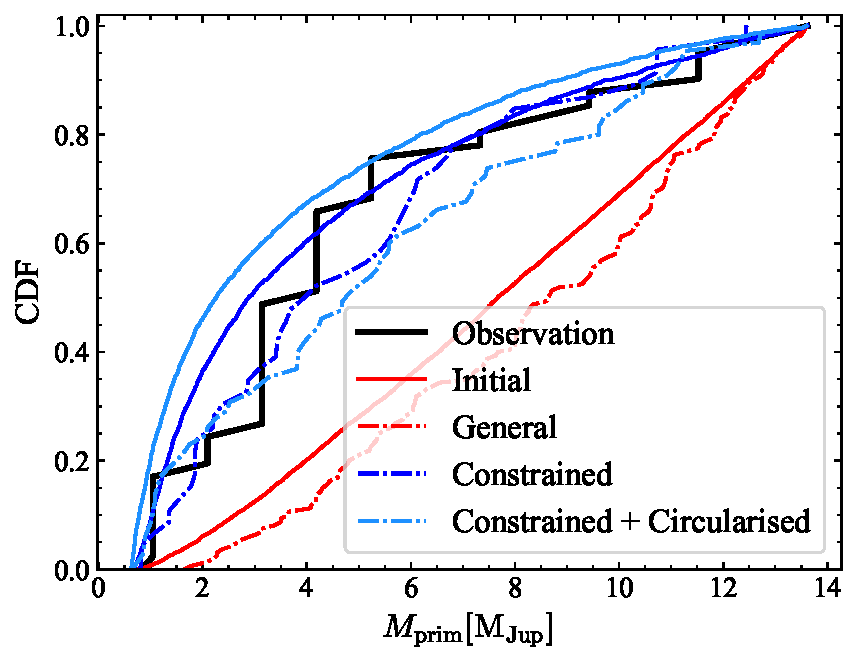
\includegraphics[width=0.75\columnwidth]{figures/Fractal_noFF_mprim_vs_obs_.pdf}
    \caption{Distribution of the primary mass of the surviving
      \jumbo\, for models Fr\_050 with an without an adapted mass
      function. The solid curves give the initial mass distribution,
      and the dashed curves the final (after 1\,Myr).  \erwan{Can we
        get rid of the light blue curve in the left panel?}}
         \label{Fig:Mdistr_F05}
\end{figure}

\section{Discussion}\label{Sect:Discussion}

We explore the possible origin of the rich population of Jupiter-mass
binary objects (\jumbos) in the direction of the Trapezium cluster.
The main problems in explaining the observations hides in the large
number of Jupiter-mass objects, their large binary fraction and the
wide separations. Assuming that they are bound, their orbits would be
soft for any encounter in the cluster, and they are not expected to
survive for more than a few hundred kyr ($\sim 0.4$\,Myr for Plummer
models, and $\aplt 0.1$\,Myr for the 0.5\,pc ${\cal ISF}$ fractal
models).

The ease at which \jumbos\, are ionized is illustrated in
figure\,\ref{Fig:Fjumbo_vs_time_model_ISF_Fr}. It may be clear that
the fractal models, due to their high frequency of strong encounters
an the earliest cluster lifetime, have difficulty preserving wide
planet-mass pairs. Plummer models are less dynamically interactive,
and the fraction of \jumbos\, remains much higher, and even relatively
wide pairs can survive.

An alternative explanation for the large population of pairs among the
free-floating Jupiter-mass objects might be that they form late.  If
\jumbos\, only formed in the last $\sim 0.2$\,Myr They have a better
chance to survive in the harsh cluster dynamical environment.  Such a
later formation would hardly affect the estimated mass of the objects,
because the cooling curves, used to estimate their mass from the
observed temperature and luminosity is rather flat at such young age
\cite{2000MNRAS.314..858L}.

The binary fraction continues to drop well after 0.2\,Myr, and by the
time the cluster is 1\,Myr old only $\sim 4$ of the binraies in the
fractal models survive. The survival fraction in the Plummer models is
considerably higher, though. The fraction of \jumbo\, continues to
drop, and by the time the cluster is $\sim 11$\,Myr the fraction of
jumbos is $\aplt 2$\,\%.  Interestingly enough,
\cite{2022NatAs...6...89M}, reported the detection of 70 to 170 single
Jupiter-mass objects in Upper Scorpius, which has an age of about
11\,Myr.  None of the objects in Upper Scorpius is paired, although
this observation could be biased in terms of missing close pairs due
to relatively low resolution of the observations.  On the other hand,
from the simulations, we would not expact many \jumbos\, in Upper
Scoprius.  The binary fraction among the Jupiter-mass objects should
be at most $\sim 2$\% . Upper Scoprius would then contain between 1
and 3\,\jumbos\, with an orbital separation $\apgt 25$\,au. So far,
none are observed.

On the other hand, our calculations, did not include primordial
stellar binaries (or higher order systems), not did we take the effect
of stellar evolution and supernovae into account. Those processes may
have a profound effect of the fraction of \jumbos, tending to reduce,
rather then increase their number.

Starting with a large population of ($\apgt 600$) single free-floating
planetary-mass objects among the stars (but without \jumbos) would
grossly underproduces the expected number of free floaters, and
consquenty fails to reproduce the observed number of \jumbos.  This
model, however, naturally leads to a mass-ratio distribution skewed to
unity, as is observed. We consider this model undesireable by the lack
of a large population of free-floating planets in the Trapezium
cluster. This could indicate the existence of a large population of
unobservable low-mass objects, but we consider this a rather exotic
possibility.

\subsection{Failure of model ${\cal SPP}$: star with a hierarchical planetary system}\label{Sect:Failure_SPP}

The ${\cal SPP}$ model systematically fail to reproduce the observed
population of \jumbos\, by a factor of 50 to 400. Changing the initial
distribution in semi-major axis of the inner orbit from a uniform
distribution to a logarithmic distribution reduces the formation rate
of \jumbos\, even further.

To further explore the failure of model ${\cal SPP}$, we perform an
additional series of simulations in the Plummer distribution with
virial radii of 0.25\,pc, and 0.50\,pc.  According to
\cite{2023arXiv231006016W}, the eventual orbital separation of the
\jumbo\, would be consistent with the difference in orbital separation
between the two planets when orbiting the star.  We performed
dditional simulations with a mutual separation $a_2-a_1 = 100$\,au and
$a_2-a_1 = 200$\,au, expecting those to lead to consistent results in
comparison with the observed range in orbital separation for the
\jumbos, as was argued in \cite{2023arXiv231006016W}.  The other
orbital parameters, for the planet masses, their eccentricites and
relative inclinations, in these models were identical to the other
${\cal SPP}$ models.

The results of these simulations are presented in
figure\,\ref{Fig:fjumbos_from_PP}.  The \jumbo-formation efficiency
for these models peaks for an orbital separation $a_1 \apgt 1000$\,au,
but steeply drops for smaller values of $a_1$.  From a total of 45
calculations with various ranges of $a_1$ and $a_2$, 39 produced a
total of 910 \jumbos.  The eventual distribution in separations is
somewhat wider than claimed by \cite{2023arXiv231006016W}, who argued
that the initial orbital distance $a_2-a_1$ would be preserved, but
reasonably wise not inconsistent with the results of
\cite{2023arXiv231006016W}.

\begin{figure}
    \centering
        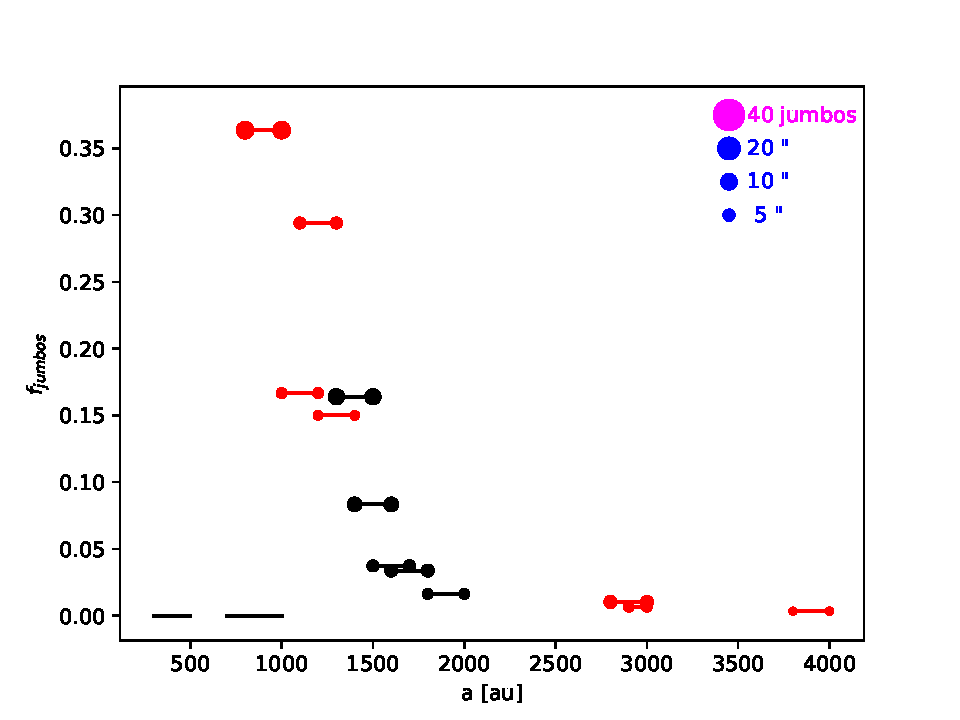
\includegraphics[width=.75\columnwidth]{figures/fig_fjumbos_from_psystems.pdf}
        \caption{The number of jumbo's produced in model ${\cal SPP}$,
          as fraction of the number of free floating planets for
          various simulations starting with a Plummer sphere with a
          virial radius of 0.5\,pc.  The bullet points along each line
          correspond with the adopted orbital separation of the two
          planets ($a_1$ and $a_2$).  The red symbols indicate an
          average orbital separations for the jumbos between 25\,au
          and 380\,au.  The symbol sizes give the number of \jumbos\,
          in these simulation linearly scales with a maximum of 9.  }
         \label{Fig:fjumbos_from_PP}
\end{figure}

The rate, derived by \cite{2023arXiv231006016W}, however, appears to
be orders of magnitude smaller than they expected.  They calculate the
rate by means of 4-body scattering experiments, in which a star with
two equal-mass planets with semi-major axes $a_1$ for the inner and
$a_2$ for the other planet, encounters a single star. Their largest
cross section of roughly $a_1^2$ is obtained if the encounter velocity
$0.8v_\star/v_1$. For an encounter at the cluster's velocity
dispersion, the inner planet would then have a orbital separation of
$\sim 900$\,au around a 1\,\MSun\, star.

Note that an inner orbital separation of $a_1=900$\,au for a
10\,\MJup\, planet leads to a Hill radius of about 160\,au. An orbit
with $a_2=1100$\,au, is then rather unstable.  Still, even in the runs
where we use these parameters the total number of \jumbos\, remains
small compared to the number of free floaters.  A stable hierarchical
system of two Jupiter-mass planets in a circular orbit around a
1\,\MSun\, star, would be dynamically stable if $a_1 \simeq 120$\,au
and $a_2 \simeq 210$\,au. Even if each star in the Trapezium cluster
was born with two such planets at most one third of the 42 observed
\jumbos\, could conceivably be explained, and the number of free
floating JMOs would run in the thousands.

The results of the cross section calculations performed by
\cite{2023arXiv231006016W} are consistent with our direct N-body
simulation, but that the adopted initial orbital separation is too
wide in comparison with a realistic population of inner planetary
orbits for Jupiter-mass objects.  Observational selection effect in
finding $\apgt 900$\,au JMOs are quite severe, but we consider it
unrealistic to have 300 out of 2500 stars to be orbited by such wide
planetary systems. In particular, when one considers the small sizes
of the observed disks in the Trapezium cluster, which today are all
smaller than 400\,au \cite{2005A&A...441..195V}.

%%The calculation os  \cite{2023arXiv231006016W} were performed using isolated scattering e
%%\cite{2023arXiv231015603C} adopt scattering experiments to determine
%%the formation rate of jumbos from their adopted initial conditions.

\subsection{Failure of model ${\cal FFC}$: Free-Floating Jupiter-Mass Objects}\label{sect:FFC_model_results}

In scenario, $\mathcal{FFC}$, we initialize $600$ to $10^4$ single
Jupiter-mass objects in a cluster of stars without \jumbos\, (see
section\,\ref{Sect:FFC}), expectating that some soft pairs form
naturally through interactions with the stars. Soft binary formation,
through three-body interactions is not expected to be very effective
\cite{1976A&A....53..259A}, but with a sufficiently large population,
one might expect a few \jumbos\, to form.  Potentially, some of the
observed \jumbos\, originate from this process.

A \jumbo\, can form in models ${\cal FFC}$, when two JMO and a single
star happen to occupy the same phase space volume, in which case the
star can escape with the excess angular momentum and energy, leaving
the two planet-mass objects bound.  The distance at which a JMO with
mass $m$ and a star with mass $M$ can be considered bound can be
estimated from the $90^\circ$ turn-around distance, which is $r_{90} =
G(M+m)/v^2$.  For our adopted clusters $r_{90} \simeq
900$\,au. Following \cite{1976A&A....53..259A}, we estimate the
probability of this to happening at $\sim 10^{-2}$ per JMO per
relaxation time. The relaxation time of our Trapezium model cluster is
approximately $t_{\rm rlx} \propto N/(6\ln(N)) t_{\rm cross} \sim
64t_{\rm cross}$. With a crossing time of about 1\,Myr (roughly the
crossing time for our 1\,pc models) we expect $\sim 0.5$ \jumbos\, to
form. The estimates by \cite{1976A&A....53..259A} adopted equal mass
objects, but the more detailed numerical study, carried out by
\cite{2011MNRAS.415.1179M}, arrive at a similar number of soft
binaries. The latter study, however, focused on post core collapsed
clusters, which is not appropriate for our Plummer models, but more in
line with our fractal models. Stellar sub-clumps collapse in the
fractal models within $\sim 0.2$\,Myr, mimicking the post collapse
evolution as addressed in \cite{2011MNRAS.415.1179M}. In principle,
their model, therefore, is somewhat appropriate to our ${\cal FCC}$
  models.

Interestingly enough, the ${\cal FFC}$ models produce quite a rich
population of stellar pairs ($82.8\pm 6.6$) and several cases where a
JMO is captured by a star ($6.5\pm3.3$) for the Plummer as well as for
the fractal models. But no \jumbos\, formed. In higher abundance of
stellar pairs compared to planetary captures is somewhat unexpected.
In figure\,\ref{Fig:eccentricity_FFC_Fr025} we present the cumulative
distribution of the eccentricities found in several of our model
calculations. Each of them is consistent with the thermal distribution
(indicated as the black dotted curve).

\begin{figure}
    \centering
        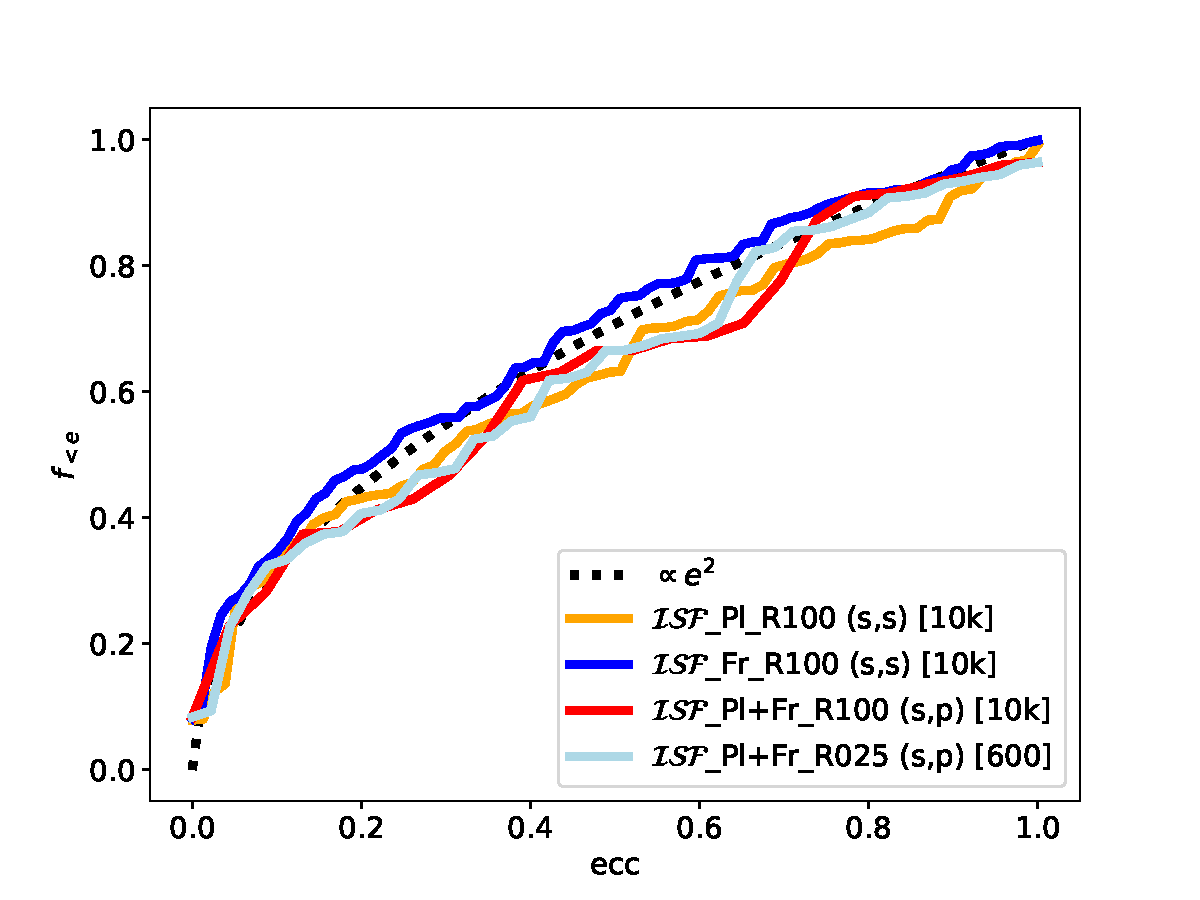
\includegraphics[width=0.75\columnwidth]{figures/fig_eccentricity_FFC.pdf}
        \caption{Eccentricity distribution for several models
          (indicated in the lower right inset) for stellar binaries and
          captured planet-mass objects. Overplotted, for comparison,
          is the thermal distribution.}
         \label{Fig:eccentricity_FFC_Fr025}
\end{figure}

The secondary masses in the stellar pairs that formed are
statistically indistinguishable from the primary masses of the stars
that captured a planet, and their orbits a wider; $182\pm67$\,au for
the binaries and $288\pm164$\,au for the captured JMOs.  With the
higher masses the binaries are roughly 100 times harder than the JMO
captured systems; straddling the hard-soft boundary.

\subsection{The long-term surviveability if \jumbos}

To study the long-term survivability of \jumbos\, we continue 5 runs
for each of the models ${\cal ISF}$\_Pl\_050 and ${\cal ISF}$\_Fr\_050
until an age of $10$\,Myr.  Our aim is to look at the survival of
\jumbos\, in older systems systems, such as Upper Scoprius. Overall,
the \jumbo\, survival rate decreases rapidly, with a half-life time
$<1$\,Myr, and the survivers have tighter orbits.  The population of
\jumbos\, eventually settles at a population of dynamically hard
pairs, in which case the mean orbital separation $\langle a\rangle
\aplt 20$\,au for two $3\, M_{\mathrm{Jup}}$ objects. The hardness of
these pairs is mostly the result of the decrease in the cluster
density with time, rather than in the shrinking of the surviving
\jumbos.

In figure\,\ref{Fig:SimTime_MPrimQ} we present the distribution in
primary mass and mass ratio for simulation ${\cal ISF}$\_F050ff at an
age of 10\,Myr (adopting the power-law primary mass function). The
younger equivalent, at an age of 1\,Myr and adopting a flat mass
function for the primaries is presented in the left panel of
figure\,\ref{Fig:Gen_mdistr_Fractal}.  The most likely survivors have
high primary and secondary masses, as could be expected based on the
hardness of these systems, which is seen in
figure\,\ref{Fig:SimTime_MPrimQ}.

\begin{figure}
    \centering
    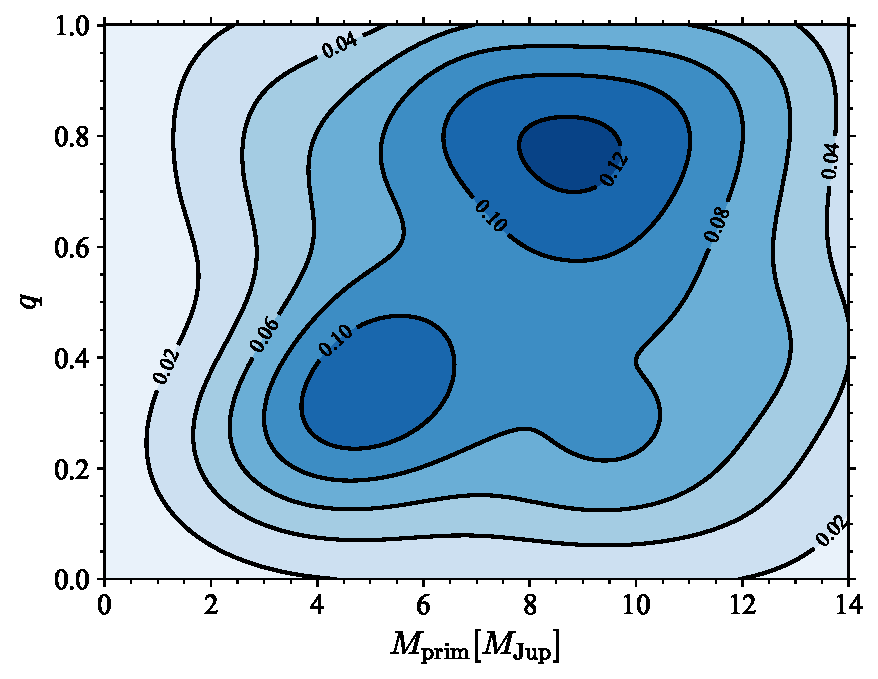
\includegraphics[width=0.75\columnwidth]{figures/Fractal_rvir0.5_FF_10Myr_mass_distr.pdf}
    \caption{Distribution of primary mass versus the mass ratio for
      model ${\cal ISF}$\_Fr\_050ff at an age of 10\,Myr.  Note that
      here we adopted the power law ($\alpha = -1.2$) mass function
      for the primaries.  Red crosses denote where observed \jumbos\,
      lie.}
         \label{Fig:SimTime_MPrimQ}
\end{figure}

\subsection{Observational Constraints}

\erwan{This paragraph still needs work, and maybe it would be merged with the next paragraph}

When fine-tuning the initial conditions, $f_{\mathrm{surv}}$ and $e$
barely changes while $a$ shows only marginal changes.  This slight
increase in $f_{r_{ij}\geq25\ \mathrm{au}}$, $\langle a\rangle$ and
$\langle r_{ij}\rangle$ could be attributed to the reduction of JMO
and \jumbos\, present in the environment and the smaller masses they
occupy making it harder for them to ionize binaries. The difference in
the semi-major axis distribution between models Fr\_050 with \jumbos\,
initially on eccentric or circular orbits, is shown in figure
\ref{Fig:Semi_Fractal}. The Fractal models exhibit a natural tendency
for trimming out wide binaries.
    
\begin{figure}
    \centering
    %%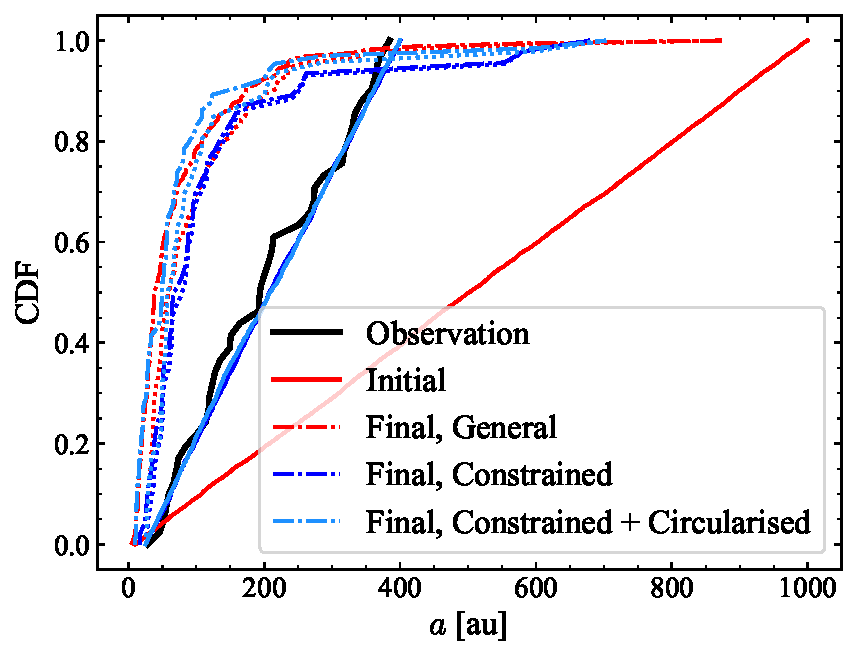
\includegraphics[width=0.49\columnwidth]{figures/Fractal_noFF_sem_axis.pdf}
    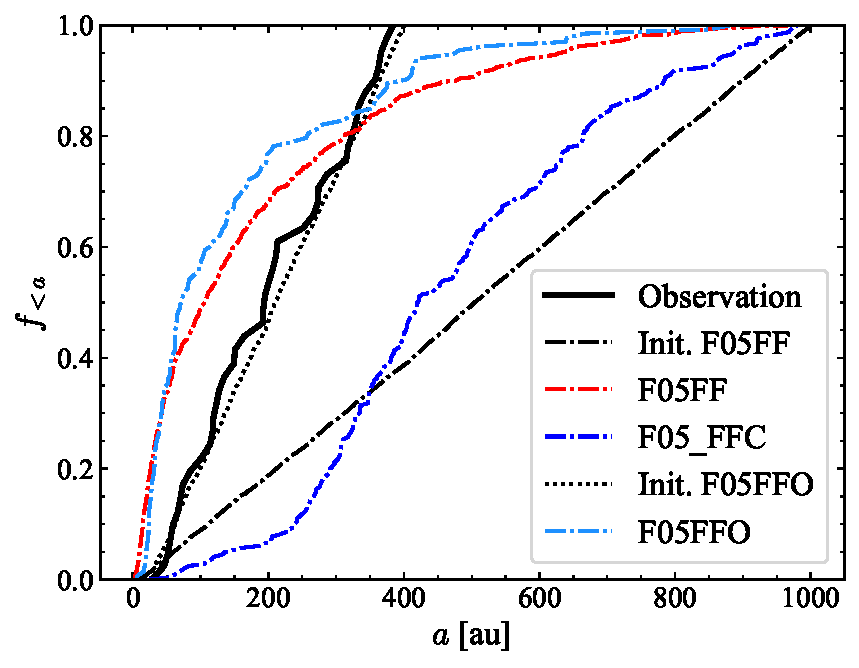
\includegraphics[width=0.49\columnwidth]{figures/Fractal_FF_sem_axis_crop.pdf}
    \caption{Cumulative distributions for the orbital separation for
      the models Fr\_050ff.
      \erwan{I am not 100\% sure what this plot shows. Is it the distro from fractals at 0.2Myr?}
    }
         \label{Fig:Semi_Fractal}
\end{figure}

No matter the initial configuration of \jumbos, a similar evolution is
observed where surviving \jumbos\, tend to have larger primary
masses. However, unlike the F05 model, the constrained model,
initialised with $\alpha = -1.25$, end up being roughly uniform in
primary mass compared to the somewhat thermal appearance for F05. In
doing, the median primary masses shift towards lower values while the
mass ratio towards larger one. A fact reflected by the statistics
shown in table \ref{Tab:Final_ISF_FFC_Results} and shown in figure
\ref{Fig:FractalObs_mdistr}.

Although, in this model, we aimed at reproducing the primary
mass-function and mass ratio distribution, we clearly under represent
high mass primaries witha low mass ratio. For the Plummer models it
will be relatively streightforward to reproduce both populations (the
high mass ratio, as well as those with a low mass ratio), but in the
fractal models the survival rate is too low to still reflect the
initial conditions.

   \begin{figure}
    \centering
    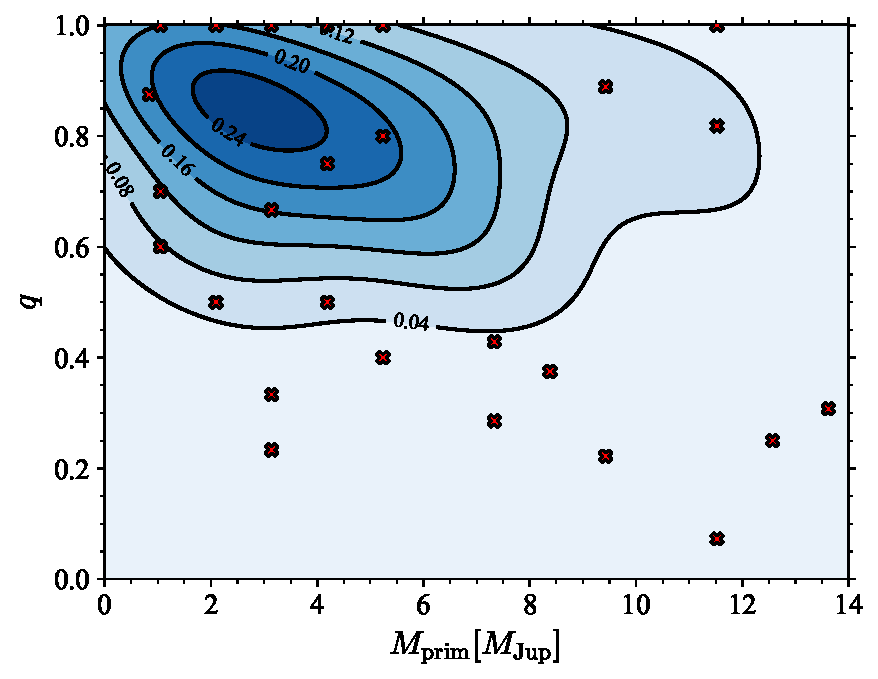
\includegraphics[width=0.75\columnwidth]{figures/Fractal_rvir0.5_Obs_mass_distr.pdf}
    \caption{Contours of constant density in the plane of primary mass
      versus mass-ratio for model $\mathcal{ISF}$\_050ff. Red crosses
      denote where observed \jumbos.  In this model, the initial mass
      function and mass-ratio distributions for the \jumbos\, were
      skewed to lower mass primararies ($\alpha = -1.2$), and to equal
      mass systems ($q$ between 0.2 and 1.0 from the thermal
      distribution.  }
         \label{Fig:FractalObs_mdistr}
   \end{figure}

The statistics of merging scenarios, and the emergence of both
Jupier-mass - Stellar binary systems and $N\geq3$ systems are
summarised in table \ref{Tab:Systems}.

In figure \ref{Fig:MixedSys_OrbParams}, we present the distribution of
the surviving \jumbos\, in semi-major axis and eccentricity. The
stellar binaries occupy roughly the same space.  The parameter space
is widely covered, with signs of low-eccentricity but very wide
($a\geq700$ au) binaries. Nevertheless, the vast majority exhibit
large eccentricities and semi-major axis, reflecting their dynamical
origin. The non-negligible amount of these systems emerging provide an
interesting prospect of detecting ultra-cold Jupiters orbiting stars
who have recently fostered them.

   \begin{figure}
    \centering
    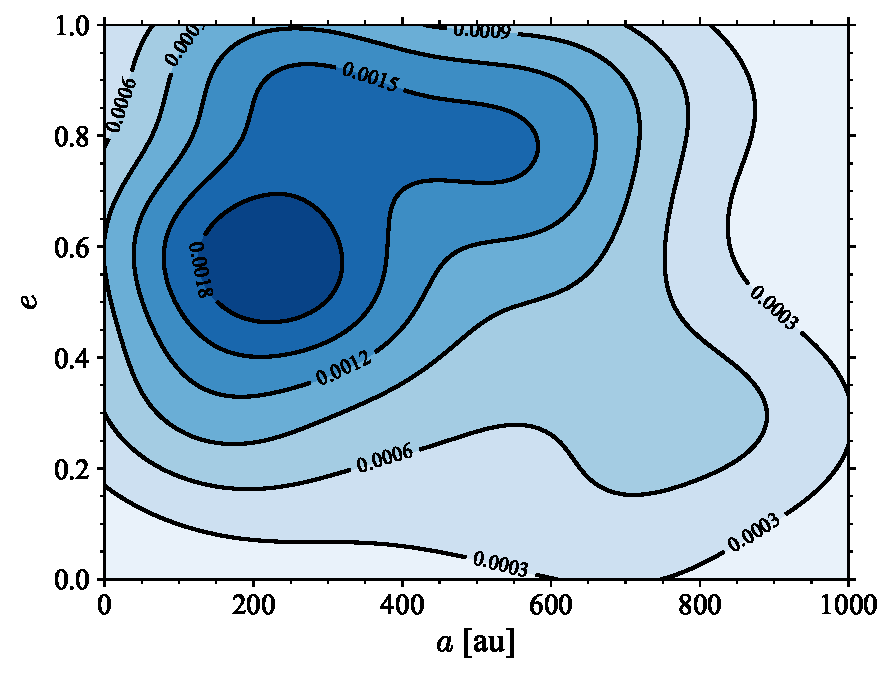
\includegraphics[width=0.75\columnwidth]{figures/Fractal_rvir0.5_FF_Obs_sem_ecc_mixed_systs.pdf}
    \caption{Contours of constant density for semi-major axis and
      eccentricities for stars that managed to capture a JMO for model
      $\mathcal{ISF}$\_050ff. These systems are suprisingly common in
      our simulations, and they even tend to be rather tight. The
      actual orbits are still dynamicall soft, though.. }
         \label{Fig:MixedSys_OrbParams}
   \end{figure}

    Given the poor reproducability in ratios of \jumbos\, to JMO free floaters and the tight orbits of \jumbos\, we conclude that the $\mathcal{ISF}$ models are most likely not the origins of \jumbos, lending us to our final possible scenario, $\mathcal{FFC}$.

   

    \begin{table}
      \caption{TO CHECK \erwan{I thikn that this table can go}.
       }
        \label{Tab:M2Events} 
        \centering 
        \begin{tabular}{c c c c c}
        \hline\hline
        Model & $\langle N_{\mathrm{JS, merge}}\rangle$ & $\langle N_{\mathrm{SS, merge}}\rangle$ & $\langle N_{\mathrm{JS}}\rangle$ &  $\langle N_{\mathrm{multi}} \rangle$ \\
        \hline \vspace{-0.75em}\\ 
           F05     & $2.5^{+0.5}_{-1.5}$ & $19^{+4}_{-7}$ & $8^{+3}_{-0}$  & $2^{+0}_{-0}$ \vspace{0.25em}\\
           F05FF   & $5.5^{+1.5}_{-1.5}$ & $21^{+2}_{-4}$ & $14^{+1}_{-3}$ & $2^{+0}_{-0}$ \vspace{0.25em}\\
           F1      & $1.0^{+1.0}_{-0.0}$ & $14^{+3}_{-5}$ & $10^{+1}_{-3}$ & $2^{+0}_{-0}$ \vspace{0.25em}\\
           F05FFL  & $5.0^{+0.0}_{-1.0}$ & $22^{+3}_{-5}$ & $1.0^{+0.0}_{-0.0}$ & $0^{+7}_{-0}$ \vspace{0.25em}\\
           \hline \vspace{-0.75em}\\
           F05O    & $2.0^{+0.8}_{-1.8}$ & $25^{+2}_{-8}$ & $4.5^{+2.8}_{-0.5}$ & $2.0^{+0}_{-0}$ \vspace{0.25em}\\
           F05FFO  & $1.0^{+1.0}_{-0.0}$ & $17^{+3}_{-1}$ & $5.0^{+1.5}_{-1.0}$ & $1.0^{+0}_{-0}$ \vspace{0.25em}\\
           F05OC   & $0.5^{+2.3}_{-0.5}$ & $20^{+5}_{-4}$ & $4.5^{+1.5}_{-1.5}$ & $3.5^{+0}_{-0}$ \vspace{0.25em}\\
           \hline
         \hline                               %inserts single line
         \label{Tab:Systems}
        \end{tabular}
     \end{table}

Our slight preference for the fractal models stems from their natural
consequence of producing higher order hierarchical systems. Much in
the same was as the two triple \jumbos\, (Jupiter-mass Triple Objects,
JuMTO). In none of the Plummer models formed any triples, however, a
seizable fraction of primordial triples may survive: we are then back
at weighting the relative importance of initial conditions versus
dynamical evolution.


%--------------------------------------------------------------------

\subsection{Assessment on the origin of \jumbos}

In the ${\cal ISF}$ Plummer models, $\sim 61$\% of the \jumbos\, are
ionized within 1\,Myr, compared to $\sim 96$\,\% for the fractal
models.  The observed population of free floaters and \jumbos\, can
then be reproduced if the cluster was born with half the free floating
as Jupiter-mass planets and half as pairs.  The current observed
primary and secondary masses of \jumbos\, would then still reflect the
conditions at birth, but the semi-major axis and eccentricity
distributions would have been affected considerably by encounters with
other cluster members. These processes tend to drive the eccentricity
distribution to resemble the thermal distribution (probably with an
excess of $\apgt 0.7$ eccentricities
\cite{2000IJoMP...15..4871P}). The semi-major axes of the jumbos would
have widened, on average by approximately 5\% due to encounters with
free-floating planet-mass objects.

Alternative to a Plummer initial stellar distribution we consider
fractal distributions, which are also able to satisfactorily reproduce
the observed populations. In the fractal models, $\sim 90$\,\% of the
priordial \jumbos\, become ionized, and in principle the entire
observed populations of free-floating Jupiter mass objects and
\jumbos\, can be explained by a 100\% initial binarity among the
\jumbos. We then conclude that single Jupiter mass objects are
preferentially born in pars with a rather flat distribution in orbital
separations with a maximum of $\sim 400$\,au.  Higher order
multiplicity (triple \jumbos) form naturally from interactions between
two or more \jumbos\, in the fractal models.

This model satisfactorily explains the observed orbital separation
distribution, with a $\sim 15$\% excess of systems with a separation
$\apgt 400$\,au. We do not expect a rich population of orbits with
separation smaller than the observed 25\,au. The fraction of pairs
among the wide systems is already high, and there are simply not
enough single JMOs observed to accomodate this tight binary
population, except if a considerable fraction of the single observed
JMOs are in fact such tight binaries.

We have a slight preference for the ${\cal ISF}$ fractal models with
0.5\,pc virial radius because hierarchical triple JMOs form naturally
in roughly the observed proportion (on average $\sim 4$ triples among
$\sim 40$ pairs and $\sim 500$ single JMOs). The singles then
originate from broken-up pairs, and the trples form in interactions
between two JMO pairs.  The dynamical formation of soft triple JMOs is
quite remarkable, and observational follow-up would be of considerable
interest.

The mass function of the single JMOs then
should resemble the combined mass functions of the primary and
secondary masses of the \jumbos. The ionization probability for a
\jumbo\, does not depend on its mass, but on the chance coincidence of
meeting a star, and the majority of JMOs seem to have come from
ionized \jumbos.  

The short-periods and the small binary fraction of the fractal models
could be salvaged if the \jumbos\, form late. If the majority of the
observed population formed $\aplt 0.2$\,Myr ago, the cluster's density
profile would already have been smoothed out, leading to fewer strong
dynamical encounters. The cluster would somewhat resemble a \jumbo
-friendly Plummer-like structure. Not only would that mediate the
survival of \jumbos\, but it also would allow them to preserve their
wide orbits, as observed.

%--------------------------------------------------------------------

\section{Conclusions}\label{Sect:Conclusions}

   
The discovery of 40 relatively wide pairs and 2 triples of
Jupiter-mass objects in the Trapezium cluster emphasizes our limited
understanding of low-mass star and high-mass planet formation. In
order to derive characteristcs for their origin we performed
simulations of Trapezium-equivalent stellar clusters (2500 stars in a
virialized $0.25$\,pc to $1.0$\,pc radius) with various compositions
of Jupiter-mass objects and stars.

Models in which planets form in wide hierarchical circum-stellar
orbits (model ${\cal SPP}$), as proposed by
\cite{2023arXiv231006016W}, produce many single free floating planets,
but insufficient numbers of pairs. The ratio of single to pairs of
planet-mass objects in these models is too low by a factor of 50 to
400, irrespective of the initial stellar distribution function.

The models in which pairs of planetary-mass objects orbit stars in the
form of a planet-moon system (or binary planets, model ${\cal SPM}$),
produce a sufficent number of free-floating planetary pairs, and cover
the proper range of orbits.  In particular the models that start with
fractal initial conditions tend to produce a sufficent fraction of
\jumbos\, among free-floating objects ${\cal O}(0.1)$, which is
close to the observed value of $0.078\pm0.012$. In the Plummer
distribution, the number of stars that survive with at least one
planet-mass objects is considerable. In general, these models predict
low-eccentricities ($e\aplt 0.4$), whereas others lead to thermalized
distributions ($e\apgt 0.6$).

For model ${\cal SPM}$ to produce a sufficient number of \jumbos\, it
requires planet-moon pairs to form in $\apgt 900$\,au orbits around
their parent star. Such wide orbits are exotic considering the fact
that the circum-stellar disks observed in the Trapezium cluster tend
to be smaller than 400\,au. We therefore do not see how such wide
planet-moon pairs can form around stars. If, however, such
binary-planets, are found in the Trapezium cluster we do consider this
model a serious candidate for producing \jumbos.  Investigating some
of the observed \jumbos\ in the images published in
\cite{2023arXiv231001231P}, we do get the impression that some
\jumbos\, may have nearby stars, but a thorough statistical study to
confirm this correlation is necessary.  Model ${\cal SPM}$ can easily
be confirmed or ruled out by establishing the existence of those left
over (or dynamically formed) planetary systems.

Ruling out models ${\cal FFC}$, ${\cal SPP}$, and possibly ${\cal
  SPM}$, we are left with the simplest solution; \jumbos\, form
together with the single stars in the cluster.  This model reproduces
the observed rates and orbital characteristics (a bit by construction,
though), it can also be used to further constrain the initial
conditions of the cluster as well as the \jumbos.

Single free floating planetary objects were discovered in abundance
(between 70 and 170 candidates) before in the Upper Scorpius
association \cite{2022NatAs...6...89M}, but these were considered to
be single free floaters.  With an age of about 11\,Myr
\cite{2022NatAs...6...89M}, Upper Scoprius is expected to be rich in
single Jupiter-mass free floating planets, but binaries will be rare
as the majority will be ionized. We still could imagine that a few
\jumbos\, have survived until today.

Finally, we would like to comment briefly on the nature of the objects
observed. We wonder that, if these objects formed in situe, and
therefore not around a star, they would be deprived of a rocky core.
\jumbos\, and JMOs would then more resemble a star in terms of the
structure, rather than a planet. This may have interesting
consequences on their dynamics, their evolution, and when they
encounter another star (collisions in our simulations are relatively
frequent). In those terms, we also wonder to what degree the term
``planet'' is rectified at all, and maybe it is time to revive the IAU
discussion on the definition of a planet.

We tend to prefer model ${\cal ISF}$ with a 0.5\,pc Plummer sphere
because it can be tuned rather easily to reproduce the observed
population of \jumbos\, and JMOs. On the other hand, we also consider
the equivalent fractal model a good candidate. We had greater
difficulty reproducing the observed \jumbos\, but they naturally lead
to some Jupiter-Mass Triple Objects (JuMTOs).  To make the fractal
model work, we can prefer \jumbos\, to form relatively late compared
to the other stars in the cluster.

\section*{Software used for this study}

In this work we used the following packages: \texttt{python}
\cite{10.5555/1593511}, \texttt{AMUSE} \cite{2018araa.book.....P},
\texttt{numpy} \cite{Oliphant2006ANumPy}, \texttt{scipy}
\cite{2020SciPy-NMeth}, \texttt{matplotlib}
\cite{2007CSE.....9...90H}.

\section*{Energy Consumption}

\erwan{We'll have to rewrite this.}

The $820$ simulations conducted during this investigation had a total
wall-clock time of $432$ days. For the XYZ runs, each CPU used $6$
cores, for the other two configurations $18$ cores were used per
CPU. In total, the CPU time for all simulations was $7680$
days. Assuming a CPU consumption rate of $12$ Watt hr$^{-1}$
\cite{2020NatAs...4..819P}, the total energy consumption is roughly
$2210$ kWh. For an emission intensity of $0.283$ kWh kg$^{-1}$
\cite{doi:10.1002/cpe.3489}, our calculations emitted $7.8$ tonnes of
CO2, roughly equivalent to two round trips by plane New York -
Beijing.

\section*{Acknowledgments}
We are grateful to Veronica Saz Ulibarrena, Shuo Huang, Maite Wilhelm,
Brent Maas, and Samuel Pearson for being available to discussing
\jumbos\, with us.
We thank NOVA for support.

\input /home/spz/Latex/lib/bib/references
% for the bibliography, at the end
%\bibliographystyle{SciPost_bibstyle.bst}
%\bibliography{references.bib} % your references Yourfile.bib

\begin{appendix}
  \section{Similarity between $r_{ij}$ and $a$}\label{Appendix:A}

  The comparison between simulations and observations is somewhat
  hindered by the different perspecitves. Whereas dynamicists prefer
  to use Kepler orbital elements, from an observational perspective
  such data is not always available. In our current study, we try to
  compare populations of binaries with observed objects. The latter
  are projected separations, which do not directly translate in
  orbital elements without full knowledge of the 6-dimension phase
  space of the orbit. We therefore have to compare projected separation
  with what we prefer to use, the semi-major axis of a bound two body
  orbit.

  Figures \ref{Fig:Plummer_rsep} and \ref{Fig:Fractal_rsep} motivate
  our choice of analysing results in terms of the semi-major axis
  given the similarity between the curves.  In all cases, $r_{ij}$
  exhibits longer tails at shorter separations/orbits. However, these
  differences are so small, especially in the fractal case, and
  considering the width of the distribution (illustrated with the
  large values for the quartile intervals) we can safely interchange
  between one and the other. In doing so, we assume that the observed
  projected separation of \jumbos\, are equivalent to their semi-major
  axis, easing our discussion.
    
    \begin{figure}
    \centering
        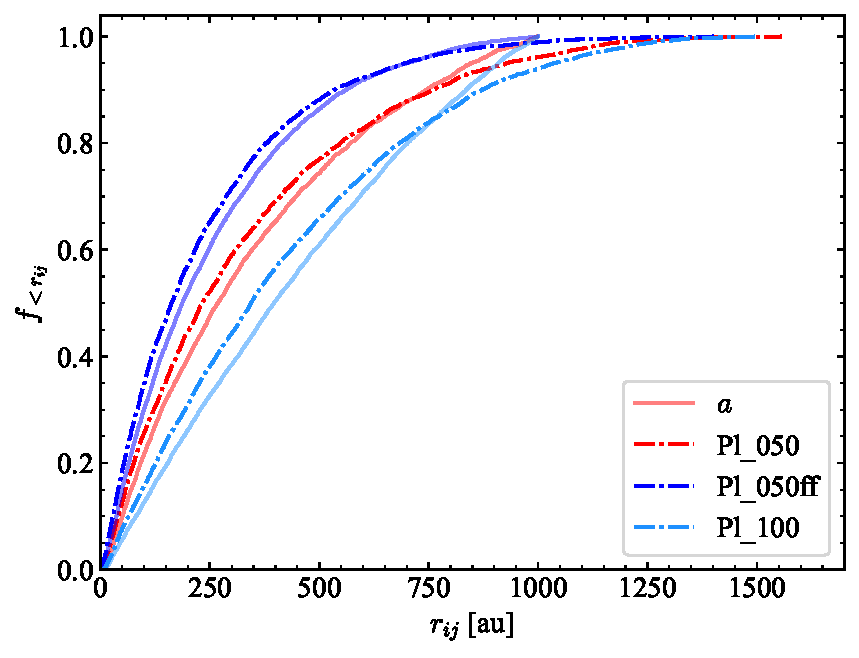
\includegraphics[width=0.75\columnwidth]{figures/Plummer_General_proj_sep.pdf}
        \caption{CDF of surviving \jumbo\, projected separation distribution for models P05, P05FF, P1. Overplotted are translucent lines denoting the respective models' \jumbos\, semi-major axis.}
         \label{Fig:Plummer_rsep}
   \end{figure}
   \begin{figure}
    \centering
        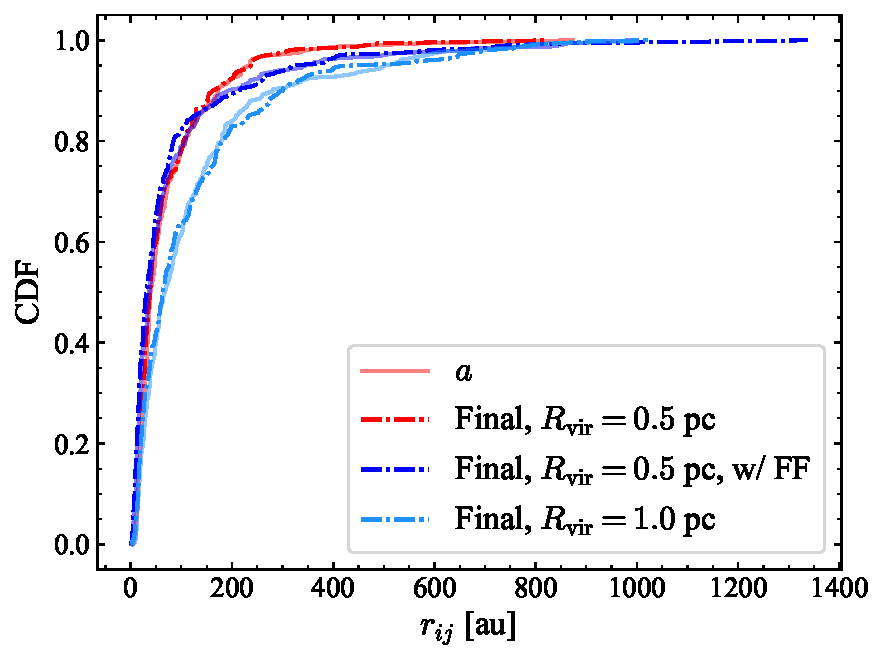
\includegraphics[width=0.75\columnwidth]{figures/Fractal_General_proj_sep.pdf}
        \caption{CDF of surviving \jumbo\, projected separation distribution for models F05, F05FF, F1. Overplotted are translucent lines denoting the respective models' \jumbos\, semi-major axis.
        \erwan{could this, and the previous figure, have the same x-axis range?}}
         \label{Fig:Fractal_rsep}
   \end{figure}
\end{appendix}
    
\end{document}
